% This file was created (at least in part) by the script ParseMdtoLatex by Louis du Plessis
% (Available from https://github.com/taming-the-beast)

\documentclass[11pt]{article}
%%%%%%%%%%%%%%%%%%%%%%%%%%%%%%%%%%%%%%%%%%%%%%%%%%%%%%%%%%%%%%%
% DO NOT EDIT THIS FILE UNLESS YOU KNOW WHAT YOU ARE DOING!!! %
%%%%%%%%%%%%%%%%%%%%%%%%%%%%%%%%%%%%%%%%%%%%%%%%%%%%%%%%%%%%%%%

% Useful packages
\usepackage[]{authblk}
\usepackage{graphicx}
\usepackage{color}
\usepackage{longtable}
\usepackage{hanging}
\usepackage{indentfirst}
\usepackage{setspace}
\usepackage{enumitem}
\usepackage{verbatim}
\usepackage{upgreek}
\usepackage{framed}
\usepackage{textcomp}
\usepackage{url}
\usepackage{soul}
\usepackage{amsmath,amsfonts,amssymb,mathrsfs}
\usepackage{fancyhdr}
\usepackage[compact]{titlesec}
\usepackage[T1]{fontenc}
\usepackage{lmodern}
\usepackage[utf8]{inputenc}
\usepackage[]{listings}
%\usepackage{fontspec}
\usepackage{placeins}
\usepackage{epstopdf}
\usepackage[export]{adjustbox}
\usepackage{tikz}
\usepackage[breaklinks]{hyperref}
\usepackage[all]{hypcap}


% References
\usepackage[backend=bibtex,hyperref=true,citestyle=authoryear,bibstyle=authortitle,firstinits=true,terseinits=true,doi=false,url=false,eprint=false,maxbibnames=10,maxcitenames=2]{biblatex}
\DeclareCiteCommand{\cite}
  {\usebibmacro{prenote}}
  {\usebibmacro{citeindex}%
   \printtext[bibhyperref]{\usebibmacro{cite}}}
  {\multicitedelim}
  {\usebibmacro{postnote}}

\DeclareCiteCommand*{\cite}
  {\usebibmacro{prenote}}
  {\usebibmacro{citeindex}%
   \printtext[bibhyperref]{\usebibmacro{citeyear}}}
  {\multicitedelim}
  {\usebibmacro{postnote}}

\DeclareCiteCommand{\parencite}[\mkbibparens]
  {\usebibmacro{prenote}}
  {\usebibmacro{citeindex}%
    \printtext[bibhyperref]{\usebibmacro{cite}}}
  {\multicitedelim}
  {\usebibmacro{postnote}}

\DeclareCiteCommand*{\parencite}[\mkbibparens]
  {\usebibmacro{prenote}}
  {\usebibmacro{citeindex}%
    \printtext[bibhyperref]{\usebibmacro{citeyear}}}
  {\multicitedelim}
  {\usebibmacro{postnote}}

\DeclareCiteCommand{\footcite}[\mkbibfootnote]
  {\usebibmacro{prenote}}
  {\usebibmacro{citeindex}%
  \printtext[bibhyperref]{ \usebibmacro{cite}}}
  {\multicitedelim}
  {\usebibmacro{postnote}}

\DeclareCiteCommand{\footcitetext}[\mkbibfootnotetext]
  {\usebibmacro{prenote}}
  {\usebibmacro{citeindex}%
   \printtext[bibhyperref]{\usebibmacro{cite}}}
  {\multicitedelim}
  {\usebibmacro{postnote}}

\DeclareCiteCommand{\textcite}
  {\boolfalse{cbx:parens}}
  {\usebibmacro{citeindex}%
   \printtext[bibhyperref]{\usebibmacro{textcite}}}
  {\ifbool{cbx:parens}
     {\bibcloseparen\global\boolfalse{cbx:parens}}
     {}%
   \multicitedelim}
  {\usebibmacro{textcite:postnote}}

\newcommand{\citep}{\parencite}
\newcommand{\citet}{\textcite}
\defbibheading{relevref}[\refname]{\section*{Relevant References}}

\renewcommand{\postnotedelim}{\iffieldpages{postnote}{\addcolon}{\addcomma\space}} 
\DeclareFieldFormat{postnote}{#1} 

\DeclareFieldFormat[article, inbook, incollection, inproceedings, patent, thesis, unpublished]{title}{#1}
\DeclareFieldFormat[article, inbook, incollection, inproceedings, patent, thesis, unpublished]{journaltitle}{\mkbibemph{#1}\nopunct}
\DeclareFieldFormat[article, inbook, incollection, inproceedings, patent, thesis, unpublished]{volume}{{#1}\addcolon} %puts volume number in parens
%\DeclareFieldFormat[article, inbook, incollection, inproceedings, patent, thesis, unpublished]{year}{\mkbibparens{#1}\nopunct} %puts year in parens

\DeclareFieldFormat[article, incollection, patent, thesis, unpublished]{pages}{{\nopp#1}}

\DeclareFieldFormat{sentencecase}{\MakeSentenceCase{#1}}

\renewbibmacro*{title}{%
  \ifthenelse{\iffieldundef{title}\AND\iffieldundef{subtitle}}
    {}
    {\ifthenelse{\ifentrytype{article}\OR\ifentrytype{inbook}%
      \OR\ifentrytype{incollection}\OR\ifentrytype{inproceedings}%
      \OR\ifentrytype{inreference}}
      {\printtext[title]{%
        \printfield[sentencecase]{title}%
        \setunit{\subtitlepunct}%
        \printfield[sentencecase]{subtitle}}}%
      {\printtext[title]{%
        \printfield[titlecase]{title}%
        \setunit{\subtitlepunct}%
        \printfield[titlecase]{subtitle}}}%
     \newunit}%
  \printfield{titleaddon}}

\DefineBibliographyStrings{english}{% various adjustments to common bib entry strings
urlseen = {Accessed:},% What goes in front of the date a URL was accessed/retrieved etc.
editor = {(Ed)},%Ed – no dot, in brackets
editors = {(Eds)},% Eds – no dot, in brackets
byeditor = {(Ed.)}}% ‘Edited by’ for edited works

\DeclareNameAlias{default}{last-first}

\renewbibmacro{in:}{}

\renewbibmacro{publisher+location+date}{
  \iflistundef{publisher}
    {}
    {\printlist{publisher}%
       {\addcomma\space}%
      \iflistundef{location}
        {}
        {\printlist{location}}%
    }
}

\DeclareBibliographyDriver{article}{%
\usebibmacro{bibindex}%
\usebibmacro{begentry}%
\usebibmacro{author/translator+others}%
\newunit\newblock
\printfield{year}%
\setunit{\labelnamepunct}\newblock
\usebibmacro{title}%
\newunit
\printlist{language}%
\newunit\newblock
\usebibmacro{byauthor}%
\newunit\newblock
\usebibmacro{bytranslator+others}%
\newunit\newblock
\printfield{version}%
\newunit\newblock
%\usebibmacro{in:}% %mit in:
\usebibmacro{journal}%
\newunit\newblock
\printfield{volume}%
\newunit\newblock
\usebibmacro{byeditor+others}%
\newunit\newblock
\usebibmacro{note+pages}%
\newunit\newblock
\iftoggle{bbx:isbn}
{}%
\newunit\newblock
\usebibmacro{doi+eprint+url}%
\newunit\newblock
\usebibmacro{addendum+pubstate}%
\newunit\newblock
\usebibmacro{pageref}%
\usebibmacro{finentry}}

\DeclareBibliographyDriver{inproceedings}{%
\usebibmacro{bibindex}%
\usebibmacro{begentry}%
\usebibmacro{author/translator+others}%
\newunit\newblock
\printfield{year}%
\setunit{\labelnamepunct}\newblock
\usebibmacro{title}%
\newunit
\printlist{language}%
\newunit\newblock
\usebibmacro{byauthor}%
\newunit\newblock
\usebibmacro{bytranslator+others}%
\newunit\newblock
\printfield{version}%
\newunit\newblock
%\usebibmacro{in:}% %mit in:
\usebibmacro{booktitle}%
\newunit\newblock
\printfield{volume}%
\newunit\newblock
\usebibmacro{byeditor+others}%
\newunit\newblock
\usebibmacro{publisher+location+date}%
\newunit\newblock
\usebibmacro{note+pages}%
\newunit\newblock
\usebibmacro{pageref}%
\usebibmacro{finentry}}

\DeclareBibliographyDriver{book}{%
\usebibmacro{bibindex}%
\usebibmacro{begentry}%
\usebibmacro{author/translator+others}%
\newunit\newblock
\printfield{year}%
\setunit{\labelnamepunct}\newblock
\usebibmacro{title}%
\newunit
\printlist{language}%
\newunit\newblock
\usebibmacro{byauthor}%
\newunit\newblock
\usebibmacro{bytranslator+others}%
\newunit\newblock
%\usebibmacro{in:}% %mit in:
\usebibmacro{booktitle}%
\newunit\newblock
\printfield{volume}%
\newunit\newblock
\usebibmacro{publisher+location+date}%
\newunit\newblock
\usebibmacro{note+pages}%
\newunit\newblock
\usebibmacro{pageref}%
\usebibmacro{finentry}}




% Page margins
\setlength{\evensidemargin}{0in}
\setlength{\headheight}{0in}
\setlength{\headsep}{0in}
\setlength{\oddsidemargin}{-0.25in}
\setlength{\paperheight}{11in}
\setlength{\paperwidth}{8.5in}
\setlength{\tabcolsep}{0in}
\setlength{\textheight}{9in}
\setlength{\textwidth}{7in}
\setlength{\topmargin}{0in}
\setlength{\topskip}{0in}
\setlength{\voffset}{0in}
\parskip = 0.15in
\pagestyle{plain}
\setlength{\parindent}{0cm}

% No white space between list items
\setlist{nolistsep}

% Hyperlink setup
\hypersetup{colorlinks=true,linkcolor=linkscol,citecolor=citescol,urlcolor=urlscol}

% Settings for code blocks
\lstset{backgroundcolor=\color[rgb]{0.972,0.972,0.972},
    tabsize=4,
    rulecolor=,
        basicstyle=\scriptsize,
        upquote=true,
        aboveskip={1.5\baselineskip},
        columns=fixed,
        showstringspaces=false,
        extendedchars=true,
        breaklines=true,
        prebreak = \raisebox{0ex}[0ex][0ex]{\ensuremath{\hookleftarrow}},
        frame=single,
        showtabs=false,
        showspaces=false,
        showstringspaces=false,
        identifierstyle=\ttfamily,
        keywordstyle=\color[rgb]{0,0,1},
        commentstyle=\color[rgb]{0.133,0.545,0.133},
        stringstyle=\color[rgb]{0.627,0.126,0.941}
}

% Colour definitions
\definecolor{citescol}{RGB}{194,101,1}
\definecolor{urlscol}{RGB}{0,150,206}
\definecolor{linkscol}{RGB}{149,0,207}
\definecolor{mycol}{RGB}{25,23,191}
\definecolor{outputcol}{RGB}{34,139,34}
\definecolor{tcol}{RGB}{165,0,14}







% TODO: The rest of the file needs to be cleaned up!
%       Past this point I am not sure what is necessary or not - Louis


\DeclareMathAlphabet{\msfsl}{T1}{cmr}{m}{it}
\DeclareMathAlphabet{\msyf}{OMX}{pcr}{m}{it}
\newcommand{\alf}{\upalpha}
\newcommand{\hilight}[1]{\colorbox{yellow}{#1}}

\newcommand{\levelone}[1]{
\bigskip
\noindent{\LARGE{\textsc{#1}}}
\vspace {0.05in}
}

\newcommand{\leveltwo}[1]{
\bigskip
\noindent{\Large{\textit{#1}}}
\vspace {-1mm}
}

\newcommand{\descriptionhead}[1]{
\noindent{\textcolor{mycol}{\textbf{\textit{#1}}}}\\ \vspace{-7mm}
}

\newcommand{\dhead}[1]{
\noindent{\textbf{\textit{#1 --}}}
}

\newcommand{\exs}[1]{
\vspace{-4mm}
\begin{itemize}
\item #1 \\ \vspace{-8mm}
\end{itemize}
}


\newcommand{\nbo}[1]{{\color{red}{#1}}}


\newcommand{\stepbullet}{\noindent \textbullet \ }
\newcommand{\mi}[1]{\textbf{\textit{#1}}}


\newcommand{\levelthree}[1]{\textit{#1 --}}


%\bibliographystyle{apalike}
%\bibpunct[; ]{(}{)}{;}{a}{,}{;}


\usepackage[breaklinks]{hyperref}
\usepackage[all]{hypcap}
\hypersetup{colorlinks=true,linkcolor=linkscol,citecolor=citescol,urlcolor=urlscol}

% Some macros for software packages
\newcommand{\R}{\texttt{R} }
\newcommand{\TESS}{\texttt{TESS}}
\newcommand{\PBD}{\texttt{PBD}}
\newcommand{\DDD}{\texttt{DDD}}
\newcommand{\Laser}{\texttt{laser}}
\newcommand{\TreePar}{\texttt{TreePar}}
\newcommand{\diversitree}{\texttt{diversitree}}
\newcommand{\RevBayes}{\texttt{RevBayes}}
\newcommand{\Rev}{\texttt{Rev}}
\newcommand{\MrBayes}{\texttt{MrBayes}}
\newcommand{\BEAST}{\texttt{BEAST}}
\newcommand{\PhyloBayes}{\texttt{PhyloBayes}}
\newcommand{\PAML}{\texttt{PAML}}

\let\otheriint\iint
\let\iint\relax
\usepackage{ wasysym }







\definecolor{shadecolor}{RGB}{194,225,255}

\setlength{\tabcolsep}{5pt}
\setlength{\topmargin}{-0.4in}
\setlength{\headheight}{14.5pt}
\pagestyle{fancy}

\newcommand{\taha}[1]{{\textcolor{red}{[TAH comment: #1]}}} % TAH comment

\titlespacing{\section}{0pt}{*0}{*0}
\titlespacing{\subsection}{0pt}{*0}{*0}
\titlespacing{\subsubsection}{0pt}{*0}{*0}

\titleformat{\section}
  {\normalfont\Large\bfseries\color{mycol}}
  {\thesection}{1em}{}

\titleformat{\subsection}
  {\normalfont\large\bfseries\color{mycol}}
  {\thesubsection}{1em}{}

\titleformat{\subsubsection}
  {\normalfont\bfseries\color{mycol}}
  {\thesubsubsection}{1em}{}

% command for MrBayes command-line step
\newcommand{\cl}[1]{{\texttt{\textbf{#1}}}}
\newcommand{\colx}[1]{{\textcolor{tcol}{#1}}}
\newcommand{\mbcl}[1]{\exs{\cl{MrBayes > {#1}}}}

\newcommand{\rbprmt}{RevBayes > } 
\newcommand{\rbcl}[1]{\exs{\cl{\rbprmt{#1}}}}
\newcommand{\rbout}[1]{\exs{\cl{\textcolor{outputcol}{#1}}}}
\newcommand{\rbdn}{{\Large \symbol{126}}} % This makes a copy/pasteable tilde
\newcommand{\rbclml}[1]{\exs{\cl{\ \ \ \ \ \ \ \ \ \ \ {#1}}}}

% text box settings
% requires compiling w/ XeLaTeX
%\newfontfamily\listingsfont[Scale=1.0]{Courier New}
%\lstset{basicstyle=\listingsfont, columns=texcl}
%\defaultfontfeatures{Mapping=tex-text}


\makeatletter
\lst@CCPutMacro\lst@ProcessOther {"2D}{\lst@ttfamily{-{}}{-{}}}
\@empty\z@\@empty
\makeatother



\setlength{\topmargin}{-0.4in}
\setlength{\headheight}{14.5pt}
\pagestyle{fancy}



\definecolor{lg}{gray}{0.75}
\def\gcirc{{%
    \setbox0\hbox{$\fullmoon$}%
    \rlap{\hbox to \wd0{\hss{$\textcolor{lg}{\newmoon}$}\hss}}\box0
}}



% Add your bibtex library here
\addbibresource{master-refs}


%%%%%%%%%%%%%%%%%%%%
% Do NOT edit this %
%%%%%%%%%%%%%%%%%%%%
\begin{document}
\renewcommand{\headrulewidth}{0.5pt}
\headsep = 20pt
\lhead{ }
\rhead{\textsc {BEAST v2 Tutorial}}
\thispagestyle{plain}


%%%%%%%%%%%%%%%%%%
% Tutorial title %
%%%%%%%%%%%%%%%%%%
\begin{center}

	% Enter the name of your tutorial here
	\textbf{\LARGE Tutorial using BEAST v2.4.6}\\\vspace{2mm}

	% Enter a short description of your tutorial here
	\textbf{\textcolor{mycol}{\Large Prior-selection}}\\

	\vspace{4mm}

	% Enter the names of all the authors here
	{\Large {\em Veronika Bošková, Venelin Mitov and Louis du Plessis}}
\end{center}

Prior selection and clock calibration using Influenza A data.

%%%%%%%%%%%%%%%%%
% Tutorial body %
%%%%%%%%%%%%%%%%%

\section{Background}\label{background}

In the Bayesian analysis of sequence data, priors play an important
role. When priors are not specified correctly it may cause runs to take
very long to converge, not converge at all or cause a bias in the
inferred trees and model parameters. Selection of proper priors and
starting values is crucial and can be a difficult exercise in the
beginning. It is not always easy to pick a proper model of tree
generation (tree prior), substitution model, molecular clock model or
the prior distribution for an unknown parameter.

The molecular clock model aims to estimate the substitution rate of the
data. It is important to understand under which circumstances to use
which model and when molecular calibration works. This will help the
investigator determine which estimates of parameters can be trusted and
which cannot.

In this tutorial, we will explore how priors are selected and how
molecular clock calibration works using the H3N2 influenza A data from
the flu virus spreading in the USA in 2009.

\section{Programs used in this
Exercise}\label{programs-used-in-this-exercise}

\subsubsection{BEAST2 - Bayesian Evolutionary Analysis Sampling
Trees}\label{beast2---bayesian-evolutionary-analysis-sampling-trees}

BEAST2 is a free software package for Bayesian evolutionary analysis of
molecular sequences using MCMC and strictly oriented toward inference
using rooted, time-measured phylogenetic trees. This tutorial is written
for BEAST v2.4.6 \citep{Bouckaert2014}.

\subsubsection{BEAUti - Bayesian Evolutionary Analysis
Utility}\label{beauti---bayesian-evolutionary-analysis-utility}

BEAUti is a graphical user interface tool for generating BEAST2 XML
configuration files.

\subsubsection{Tracer}\label{tracer}

Tracer (\url{http://tree.bio.ed.ac.uk/software/tracer}) is used to
summarize the posterior estimates of the various parameters sampled by
the Markov Chain. This program can be used for visual inspection and to
assess convergence. It helps to quickly view median estimates and 95\%
highest posterior density intervals of the parameters, and calculates
the effective sample sizes (ESS) of parameters. It can also be used to
investigate potential parameter correlations. We will be using Tracer
v1.6.

\subsubsection{TreeAnnotator}\label{treeannotator}

TreeAnnotator is used to summarize the posterior sample of trees to
produce a maximum clade credibility tree. It is also useful to summarise
and visualise the posterior estimates of other tree parameters
(e.g.~node height).

\subsubsection{FigTree}\label{figtree}

FigTree (\url{http://tree.bio.ed.ac.uk/software/figtree}) is a program
for viewing trees and producing publication-quality figures. It can
interpret the node-annotations created on the summary trees by
TreeAnnotator, allowing the user to display node-based statistics
(e.g.~posterior probabilities). We will be using FigTree v1.4.2.

\section{Practical: H3N2 flu dynamics - heterochronous
data}\label{practical-h3n2-flu-dynamics---heterochronous-data}

In this tutorial, we will estimate the rate of evolution from a set of
virus sequences that have been isolated either at one point in time
(homochronous) or at different points in time (heterochronous or
time-stamped data). We use the hemagglutinin (HA) gene of the H3N2
strain spreading across America alongside the pandemic H1N1 virus in
2009 \citep{cdc2009}.

The aim of this tutorial is to obtain estimates for the:

\begin{itemize}

\item
  rate of molecular evolution
\item
  phylogenetic relationships with measures of internal node heights
\item
  date of the most recent common ancestor of the sampled virus
  sequences.
\end{itemize}

The more general aim of this tutorial is to:

\begin{itemize}

\item
  understand how to set priors and why this is important
\item
  understand why and when the rate of evolution can be estimated from
  the data.
\end{itemize}

\subsection{The Data}\label{the-data}

The full heterochronous dataset contains an alignment of 139 HA
sequences 1738 nucleotides long. The samples were obtained from
California between April and June 2009 (file named
\lstinline!InfluenzaAH3N2_HAgene_2009_California_heterochronous.nexus!).
The homochronous data is a subset of the heterochronous data, consisting
of an alignment of 29 sequences of 1735 nucleotides all sampled on April
28, 2009 (file named
\lstinline!InfluenzaAH3N2_HAgene_2009_California_homochronous.nexus!).

\subsection{Creating the Analysis File with
BEAUti}\label{creating-the-analysis-file-with-beauti}

We will use BEAUti to select the priors and starting values for our
analysis and save these settings into a BEAST-readable XML file.

\begin{framed}
Begin by starting the BEAUti program.
\end{framed}

\subsubsection{Installing BEAST 2
Plug-Ins}\label{installing-beast-2-plug-ins}

Since we will be using the birth-death skyline model (\textbf{BDSKY})
\citep{Stadler2013}, we need to make sure it is available in BEAUti. It
is not one of the default models but rather an add-on (also called a
plug-in or package). You only need to install a BEAST2 package once.
Thus, if you close BEAUti, you do not have to load \textbf{BDSKY} the
next time you open the program. However, it is worth checking the
package manager for updates to plug-ins, particularly if you update your
version of BEAST2. For this tutorial we need to ensure that we have at
least BDSKY v1.3.3 installed.

\begin{framed}
Open the \textbf{BEAST 2 Package Manager} by navigating to \textbf{File
\textgreater{} Manage Packages}. (Figure \ref{packageManage1})
\end{framed}

\begin{figure}
    \centering
    \includegraphics[width=0.750000\textwidth]{figures/beast2_package_manager_opening.png}
    \caption{Finding the BEAST2 Package Manager.}
    \label{packageManage1}
\end{figure}

\begin{framed}
Install the \textbf{BDSKY} package by selecting it and clicking the
\textbf{Install/Upgrade} button. (Figure \ref{packageManage2})
\end{framed}

\begin{figure}
    \centering
    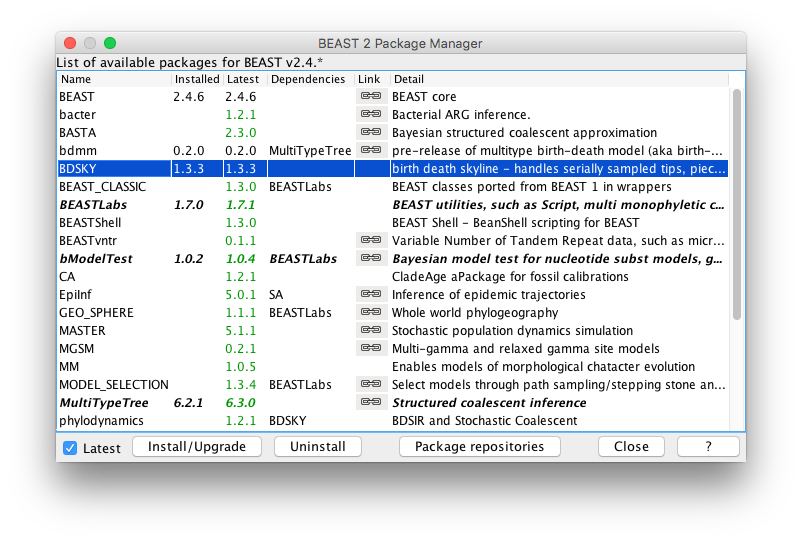
\includegraphics[width=0.750000\textwidth]{figures/beast2_package_manager.png}
    \caption{The BEAST2 Package Manager.}
    \label{packageManage2}
\end{figure}

After the installation of an add-on, the program is on your computer,
but BEAUti is unable to load the template files for the newly installed
model unless it is restarted. So, let's restart BEAUti to make sure we
have \textbf{BDSKY} model at hand.

\begin{framed}
Close the \textbf{BEAST 2 Package Manager} and \textbf{\emph{restart}}
BEAUti to fully load the \textbf{BDSKY} package.
\end{framed}

\subsubsection{Importing alignment}\label{importing-alignment}

We will first analyse the alignment of sequences sampled through time
(heterochronous sequences).

\begin{framed}
In the \textbf{Partitions} panel, import the nexus file with the
alignment by navigating to \textbf{File \textgreater{} Import Alignment}
in the menu (Figure \ref{importAlignment}) and then finding the file
called
\lstinline!InfluenzaAH3N2_HAgene_2009_California_heterochronous.nexus!
file on your computer.
\end{framed}

\begin{figure}
    \centering
    \includegraphics[width=0.750000\textwidth]{figures/beast2_import_alignment.png}
    \caption{Importing alignment into BEAUti.}
    \label{importAlignment}
\end{figure}

You can view the alignment by double-clicking on the name of the
alignment in BEAUti. Since we only have one partition there is nothing
more we can do in the \textbf{Partitions} panel and proceed to
specifying the tip dates.

\subsubsection{Setting up tip dates}\label{setting-up-tip-dates}

The heterochronous dataset contains the information on when the
sequences were sampled. We want to use this information to specify the
tip dates in BEAUti.

\begin{framed}
In the \textbf{Tip Dates} panel, click the \textbf{Use tip dates}
option.
\end{framed}

We want all the tree information to be specified for units of time in
``years'', thus we leave the \textbf{Dates specified as} option set to
default ``year''. Also we want the time to flow forward in time in the
tree, therefore, we keep to default option of tip dates being specified
as ``Since some time in the past'' (Figure \ref{timeUnitsAndFlow}).

\begin{figure}
    \centering
    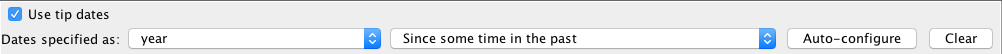
\includegraphics[width=0.750000\textwidth]{figures/beast2_time_specification.png}
    \caption{Specifying time units and direction of time flow.}
    \label{timeUnitsAndFlow}
\end{figure}

You could specify the tip dates by hand, by clicking for each row
(i.e.~for each sequence) into the \textbf{Date} column and typing the
date information in for each sequence in turn. However, this is a
laborious and error-prone procedure and can take a long time to finish.
Fortunately, we can use BEAUti, to read off the dates from the sequence
names for us. Each sequence is named such that the expression after the
last underscore character (``\_``) contains the sampling date
information. BEAUti can search for this expression to extract the
sequence date.

\begin{framed}
Press the \textbf{Guess} button. A window will appear where you can
specify how BEAUti can find the date of sampling of each sequence.
(Figure \ref{guessDates})

Select \textbf{use everything} and specify \textbf{after last} \_.
\end{framed}

\begin{figure}
    \centering
    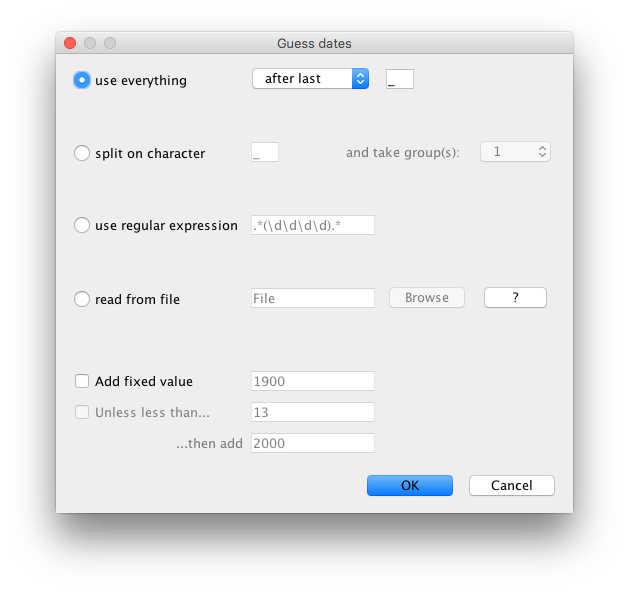
\includegraphics[width=0.750000\textwidth]{figures/beast2_guess_dates.png}
    \caption{Specifying tip dates.}
    \label{guessDates}
\end{figure}

You should now see that the tip ages have been filled in for all of the
taxa and that the \textbf{Date} columns shows a number in form 2009.xyz
and the \textbf{Height} column shows the number in form 0.abc (the
height of the tip from present time, where present is 0.0).

Now we are done with the data specification and we are about to start
specifying models and priors for the model parameters.

\subsubsection{Specifying the Site
Model}\label{specifying-the-site-model}

\begin{framed}
Navigate to the \textbf{Site Model} panel, where we can choose the model
of nucleotide evolution that we want to assume to underly our dataset.
\end{framed}

Our dataset is made of nucleotide sequences. There are four models of
nucleotide evolution available in BEAST2: JC69, HKY, TN93 and GTR. JC69
model is the simplest evolutionary model. All the substitutions are
assumed to happen with the same rate and all the bases are assumed to
have identical frequencies, i.e.~each base A, C, G and T is assumed to
have an equilibrium frequency of 0.25. In HKY model, the rate of
transitions A $ \leftrightarrow $ G and C
$ \leftrightarrow $ T is allowed to be different from the
rate of transversions A $ \leftrightarrow $ C, G
$ \leftrightarrow $ T. Furthermore, the frequency of each
base can be either ``Estimated'', ``Empirical'' or ``All Equal''. When
we set the frequencies to ``Estimated'', the frequency of each base will
be co-estimated as a parameter during the BEAST run. If we use
``Empirical'', base frequencies will be set to the frequencies of each
base found in the alignment. Finally, if set to ``All Equal'', the base
frequencies will be set to 0.25. The TN93 model is slightly more
complicated than HKY, by allowing for different rates of A
$ \leftrightarrow $ G and C $ \leftrightarrow $
T transitions. Finally, the GTR model is the most general model and
allows for different substitution rates between each pair of nucleotides
as well as different base frequencies, resulting in a total of 9 free
parameters.

\begin{framed}
\textbf{QUESTION: Which substitution model may be the most appropriate
for our dataset and why?}

You can discuss with your neighbour or with the teaching assistants if
you like. After you have made your decision, continue with the tutorial.
\end{framed}

Since we do not have any extra information on how the data evolved, the
decision is not clear cut. The best would be to have some independent
information on what model fits the influenza data the best.
Alternatively, one could perform model comparison, or apply reversible
jump MCMC (see for example the bModelTest and substBMA packages) to
choose the best model. Let's assume, we have done some independent data
analyses and found the HKY model to fit the influenza data the best. In
general, this model captures the major biases that can arise in the
analysis of the nucleotide data.

Now we have to decide whether we want to assume all of the sites to have
been subject to the same substitution rate or if we want to allow for
the possibility that some sites are evolving faster than others. For
this, we choose the number of gamma rate categories. This model scales
the substitution rate by a factor, which is defined by a Gamma
distribution. If we choose to split the Gamma distribution into 4
categories, we will have 4 possible scalings that will be applied to the
substitution rate. The probability of a substitution at each site will
be calculated under each scaled substitution rate (and corresponding
transition probability matrix) and averaged over the 4 outcomes.

\begin{framed}
\textbf{QUESTION: Do you think a model that assumes one rate for all the
sites is preferable over a model which allows different substitution
rates across sites (i.e.~allows for several gamma rate categories)? Why
or why not?}

You can again discuss with your neighbour or with the teaching
assistants if you like. After you have made your decision, continue with
the tutorial.
\end{framed}

Once again, a proper model comparison, i.e.~comparing a model without
gamma rate heterogeneity to a model with some number of gamma rate
categories, should ideally be done. We do not have any independent
information on whether gamma rate categories are needed or not. Thus, we
take our best guess in order not to bias our analyses. Since the data
are the sequences of the HA (hemagglutinin) gene of influenza, we may
want to allow for variation of the substitution rates between sites.
Hemagglutinin is a surface protein on the virus and is under significant
evolutionary pressure from the immune system of the host organism. It is
not unrealistic to assume that some sites may be under more pressure to
escape from the immune system.

Let us therefore choose the HKY model with 4 gamma rate categories for
the substitution rate.

\begin{framed}
Change the \textbf{Gamma Category Count} to 4, tick the estimate box
next to the \textbf{Shape} parameter of the Gamma distribution and set
the \textbf{Subst Model} to \textbf{HKY}. Make sure that both
\textbf{Kappa} and \textbf{Frequencies} are estimated. (Figure
\ref{substitutionModel})
\end{framed}

\begin{figure}
    \centering
    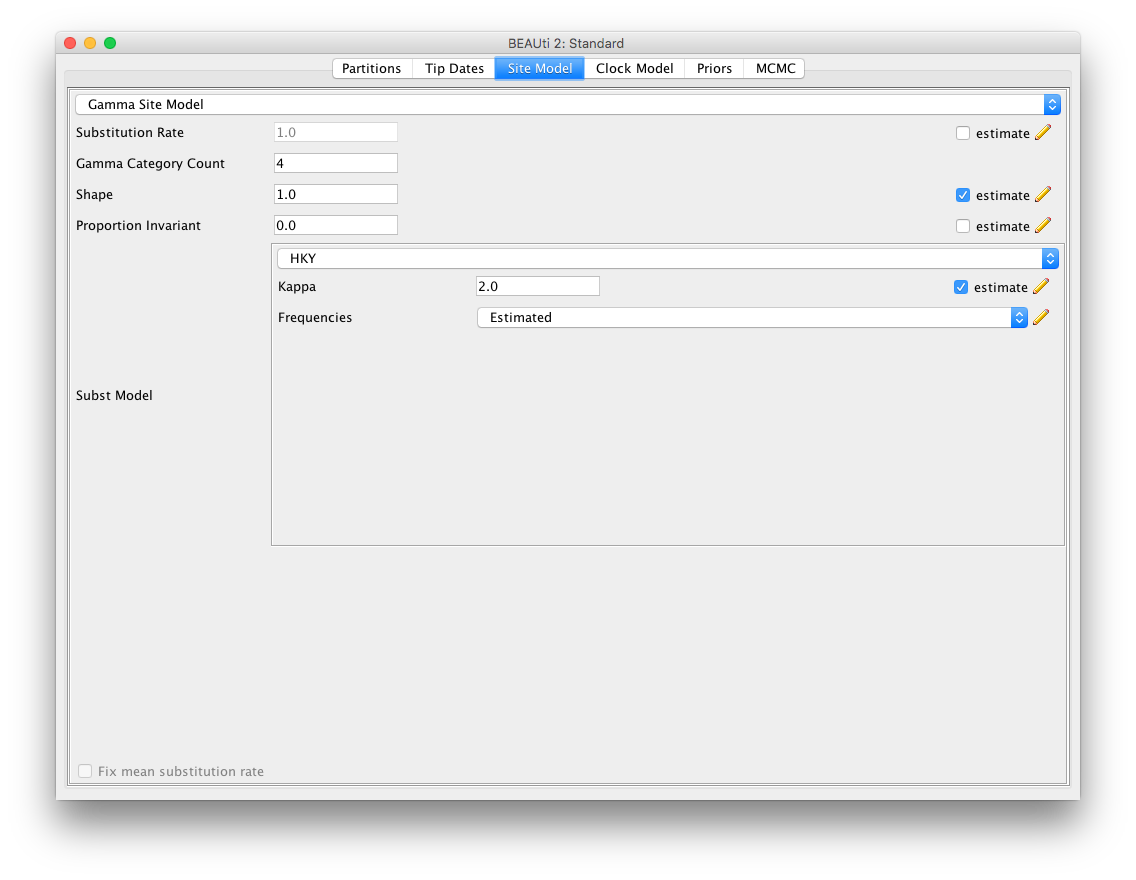
\includegraphics[width=0.750000\textwidth]{figures/beast2_substitution_model.png}
    \caption{Specifying substitution model.}
    \label{substitutionModel}
\end{figure}

Notice that we estimate the shape parameter of the Gamma distribution as
well. This is generally recommended, unless one is sure that the Gamma
distribution with the shape parameter equal to 1 captures exactly the
rate variation in the given dataset. Notice also, that we leave the
substitution rate fixed to 1.0 and do not estimate it. In fact, the
overall substitution rate is the product of the clock rate and the
substitution rate (one of the two acting as a scalar rather than a
quantity measured in number of substitutions per site per time unit),
and thus fixing one to 1.0 and estimating the other one allows for
estimation of the overall rate of substitution. We will therefore use
the clock rate to estimate the number of substitutions per site per
year.

\subsubsection{Specifying the Clock
Model}\label{specifying-the-clock-model}

\begin{framed}
Navigate to the \textbf{Clock Model} panel.
\end{framed}

Four different clock models are available in BEAST 2, allowing us to
specify lineage-specific substitution rate variation. The default model
in BEAUti is the \emph{Strict Clock}. The other three models relax the
assumption of a constant substitution rate. The \emph{Relaxed Clock Log
Normal} allows for the substitution rates associated with each branch to
be independently drawn from a single, discretized log normal
distribution \citep{drummond06}. Under the \emph{Relaxed Clock
Exponential} model, the rates associated with each branch are drawn from
an exponential distribution \citep{drummond06}. Both of these models are
uncorrelated relaxed clock models. The log normal distribution has the
advantage that one can estimate its variance, which reflects the extent
to which the molecular clock needs to be relaxed. In both models, BEAUti
sets by default the \textbf{Number Of Discrete Rates} to -1. This means
that the number of bins that the distribution is divided into is equal
to the number of branches. The last available model is the \emph{Random
Local Clock} which averages over all possible local clock models
\citep{drummond10}.

\begin{framed}
\textbf{QUESTION: Which clock model may be the most appropriate for our
dataset and why?}
\end{framed}

Since we are observing the sequence data from a single epidemic of H3N2
virus in humans in a single location (south-west of USA), we do not have
any reason to assume different substitution rates for different
lineages. Thus, the most straightforward option is to choose the default
\textbf{Strict Clock} model (Figure \ref{clockModel}). Note however,
that a rigorous model comparison would be the best way to proceed with
the choice of the clock model.

\begin{figure}
    \centering
    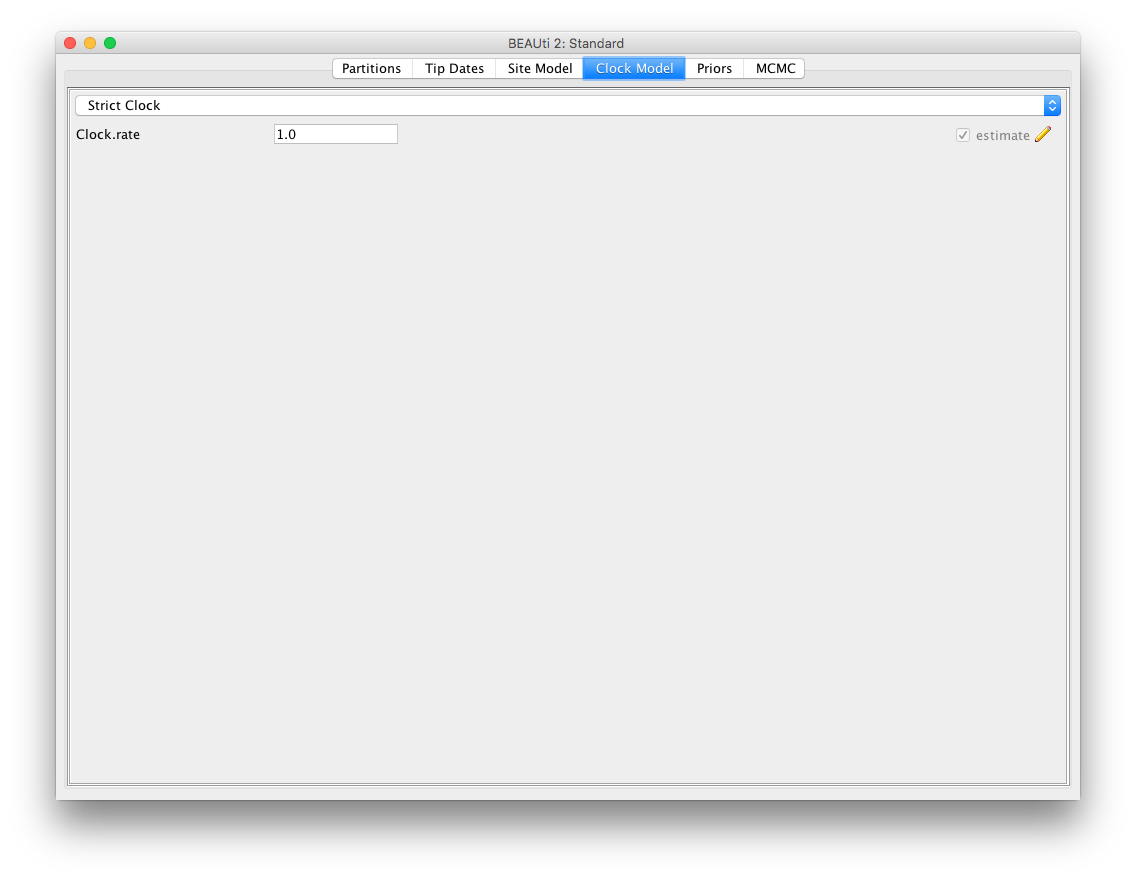
\includegraphics[width=0.750000\textwidth]{figures/beast2_clock_model.png}
    \caption{Specifying the clock model.}
    \label{clockModel}
\end{figure}

\subsubsection{Selecting Priors}\label{selecting-priors}

\begin{framed}
Navigate to the \textbf{Priors} panel.
\end{framed}

Since the dynamics of influenza virus is likely to change due to the
depletion of the susceptible population and/or the presence of the
resistant individuals, we choose the birth-death skyline model of
population dynamics with 5 time intervals for $ R_e $, to
capture this likely change of dynamics over time. $ R_0 $,
the basic reproductive number, is an important variable for the study of
infectious diseases, since it defines how many individuals a single
infected individual infects on average in a completely susceptible
population over the course of her/his infection. $ R_e $,
the effective reproduction number, is the average number of secondary
infections caused by an infected individual at a given time during the
epidemic. Thus, $ R_e $ is a function of time. In other
words, it tells us how quickly the disease is spreading in a population.
As long as $ R_e $ is above 1 the epidemic is likely to
continue spreading, therefore prevention efforts aim to push
$ R_e $ below 1. Note that as more people become infected
and the susceptible population decreases $ R_e $ will
naturally decrease over the course of an epidemic, however treatment,
vaccinations, quarantine and changes in behaviour can all contribute to
decreasing $ R_e $ faster. In a birth-death process,
$ R_e $ is defined as the ratio of the birth (or speciation)
rate and the total death (or extinction) rate. $ R_e $ for
any infection is rarely above 10, so we set this as the upper value for
$ R_e $ in our analysis.

\begin{framed}
For the \textbf{Tree} model, select the option \textbf{Birth Death
Skyline Serial}.

Then, click in the arrow to the left from \textbf{reproductiveNumber} to
open all the options for $ R_e $ settings (Figure
\ref{treePrior}). Leave all the settings to the default, since it
specifies a prior that is not too strong and centered around 1. This is
exactly what we want.

Then, click on the button where it says \textbf{initial = {[}2.0{]}
{[}0.0, Infinity{]}}. A pop-up window will show up (Figure
\ref{RePrior}).

In the pop-up window change the \textbf{Upper}, the upper limit of the
prior distribution, from Infinity to 10 and the \textbf{Dimension} of
the $ R_e $ from 10 to 5 and click \textbf{OK}.
\end{framed}

\begin{figure}
    \centering
    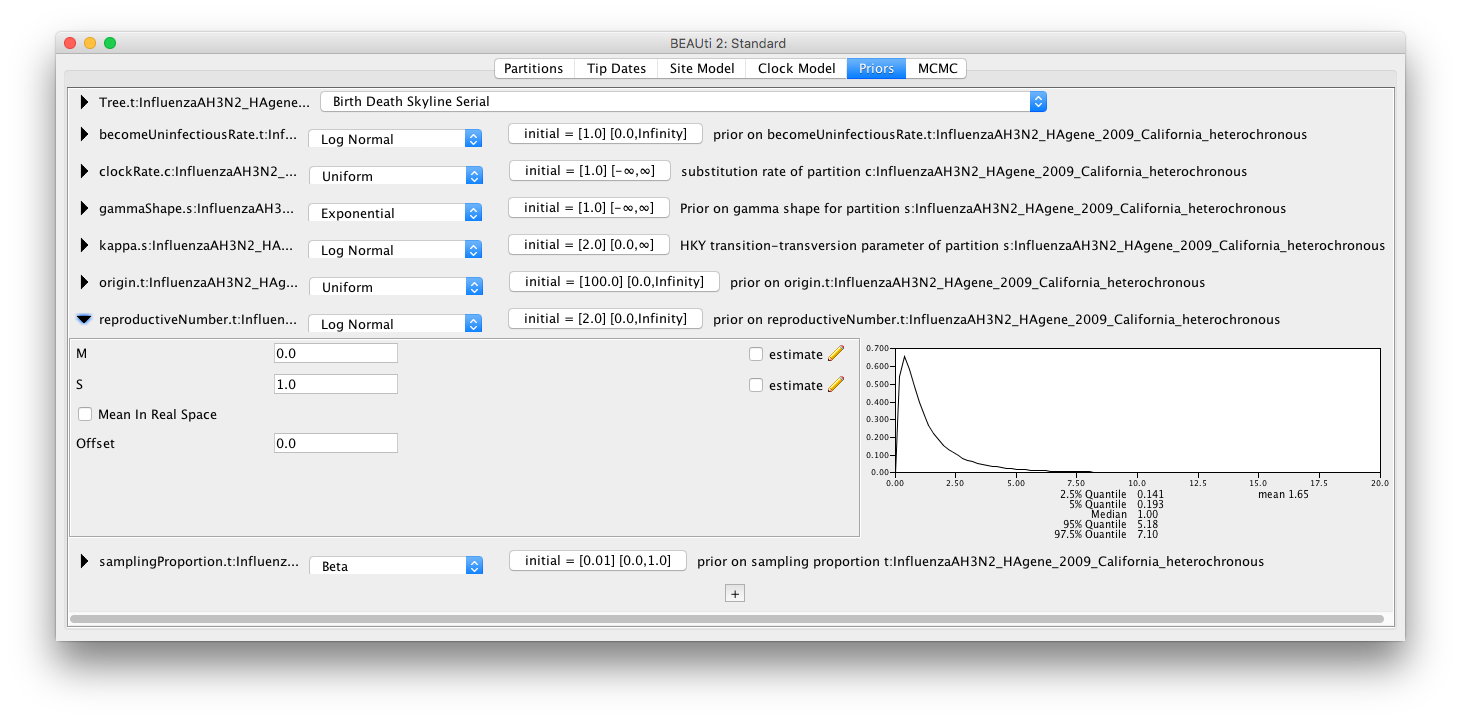
\includegraphics[max width=\textwidth, max height=0.9\textheight]{figures/beast2_prior_Re.png}
    \caption{Specifying the tree prior.}
    \label{treePrior}
\end{figure}

\begin{figure}
    \centering
    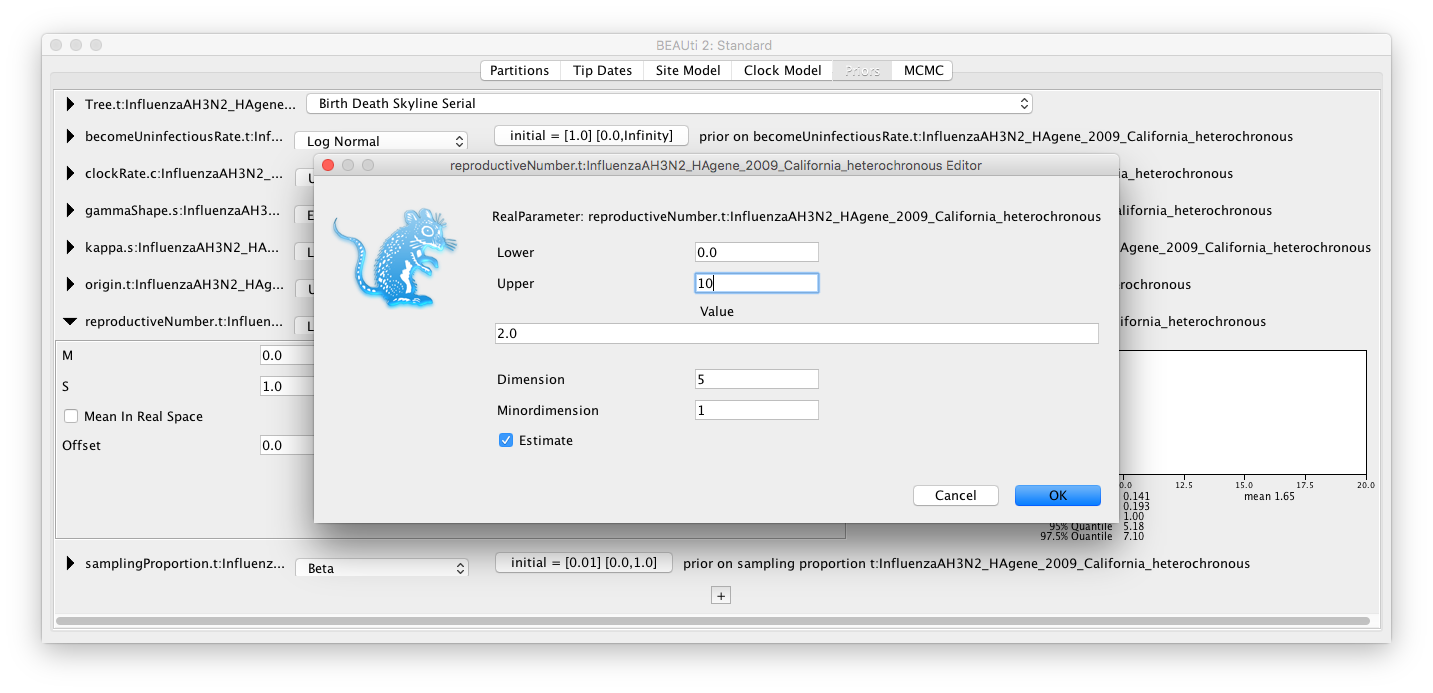
\includegraphics[max width=\textwidth, max height=0.9\textheight]{figures/beast2_prior_Redimension.png}
    \caption{Specifying the `$ R_e $` prior.}
    \label{RePrior}
\end{figure}

Notice that the pop-up window allows one to specify not only the
\textbf{Dimension} but also the \textbf{Minordimension}. If the
parameter is specified as a vector of $ n $ entries, we only
use the \textbf{Dimension} with input $ n $. If the
parameter is specified as an n x m matrix, we then use the
\textbf{Minordimension} to specify the number of columns (m) the
parameter is split into. In the birth-death skyline model, we use the
parameter vector only, and thus the \textbf{Minordimension} always stays
specified as 1. (In fact, \textbf{Minordimension} is only used very
rarely in any BEAST2 model).

After we have specified the prior for $ R_e $, the next
prior that needs our attention is the \textbf{becomeUninfectiousRate}.
This specifies how quickly a person infected with influenza recovers.
From our personal experience, we would say, it takes around one week to
10 days from infection to recovery. Since the rate of becoming
uninfectious is the reciprocal of the period of infectiousness this
translates to a becoming uninfectious rate of 365/10=36.5 to 365/7
$ \approx $ 52.14 per year (recall that we specified dates
in our tree in years, and not days). Let us set the prior for
\textbf{becomeUninfectiousRate} rate accordingly.

\begin{framed}
Click on the arrow next to \textbf{becomeUninfectiousRate} and change
the value for \textbf{M} (mean) of the default log normal distribution
to 52 and tick the box \textbf{Mean In Real Space} to specify the mean
of the distribution in real space instead of log space (Figure
\ref{becomeUninfectiousPrior}).
\end{framed}

\begin{figure}
    \centering
    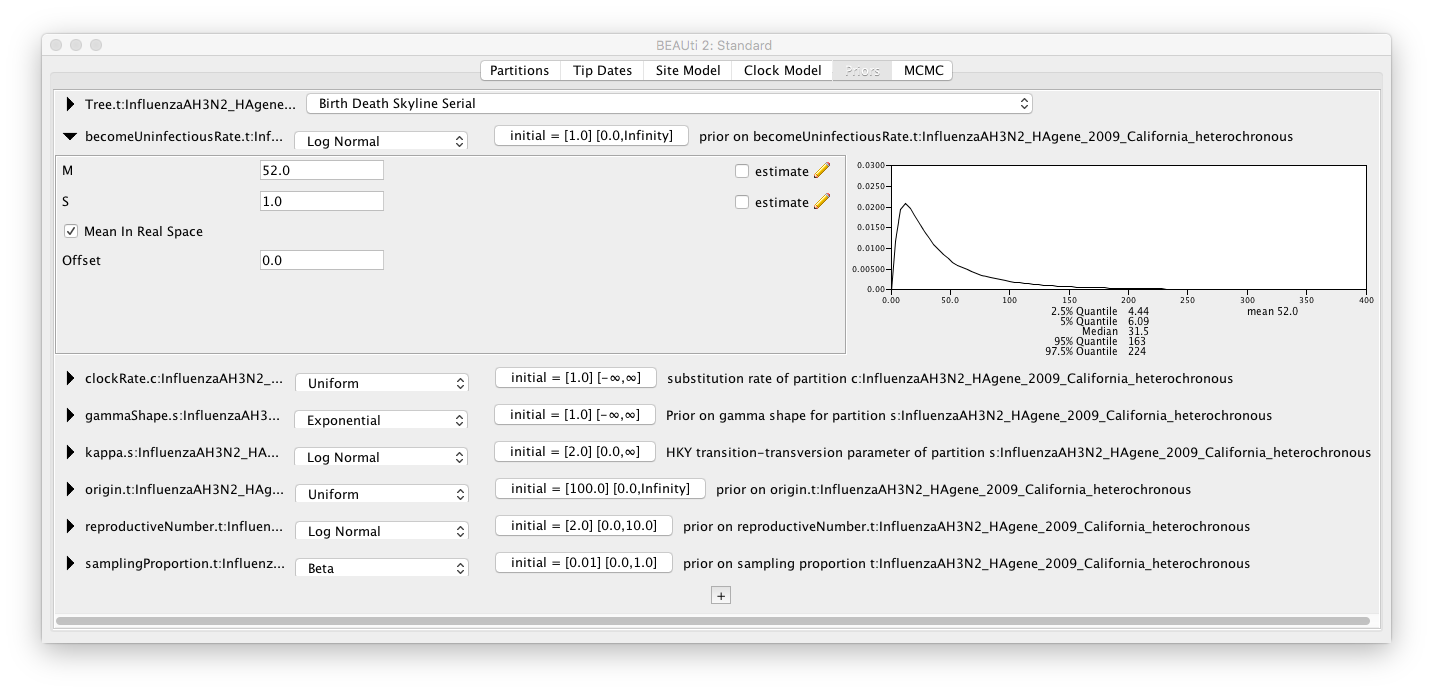
\includegraphics[max width=\textwidth, max height=0.9\textheight]{figures/beast2_prior_becomeUninfectious.png}
    \caption{Specifying the become uninfectious prior.}
    \label{becomeUninfectiousPrior}
\end{figure}

Looking at the 2.5\% and 97.5\% quantiles for the distribution we see
that 95\% of the weight of our becoming uninfectious rate prior falls
between 4.44 and 224, i.e.~our prior on the period of infectiousness is
between $ \approx $ 1.63 and 82.2 days. Thus, our prior is
quite diffuse. If we wanted to use a more specific prior we could
decrease the standard deviation of the distribution (the \textbf{S}
parameter).

Now we have to specify the clock rate prior. This is the prior for the
substitution rate.

\begin{framed}
\textbf{QUESTION: What substitution rate is appropriate for viruses?
More specifically, what substitution rate is expected for influenza
virus, in your opinion?}
\end{framed}

By default, the clock rate in BEAST2 has a uniform prior between 0 and
infinity. This is not only extremely unspecific, but also an improper
prior (it does not integrate to 1). In general, a log-normal
distribution works well for rates, since it does not allow negative
values. Furthermore, it places most weight close to 0, while also
allowing for larger values, making it an appropriate prior for the clock
rate, which we expect to be quite low in general, but may be higher in
exceptional cases. You could set your best guess as a prior by, for
example, choosing a log-normal distribution centered around your best
guess for the substitution rate.

Now consider the following information: Influenza virus is an RNA virus
\citep{kawaoka2006} and RNA viruses in general, have a mutation rate of
$ \approx $ 10$^{-3}$ substitutions per site per year
\citep{jenkins2002}.

\begin{framed}
\textbf{QUESTION: Did you change your best guess, for the substitution
rate appropriate for RNA viruses? What would it be? How would you
specify the prior?}
\end{framed}

Our best guess would be to set the prior distribution peaked around
10$^{-3}$ substitutions per site per year.

\begin{framed}
Change the prior for the clock rate from a \textbf{Uniform} to
\textbf{Log Normal} distribution. Click on the arrow next to the
\textbf{clockRate} and change the value for \textbf{M} (mean) of the
default log normal distribution to 0.001 and tick the box \textbf{Mean
In Real Space} (Figure \ref{clockRatePrior}).
\end{framed}

\begin{figure}
    \centering
    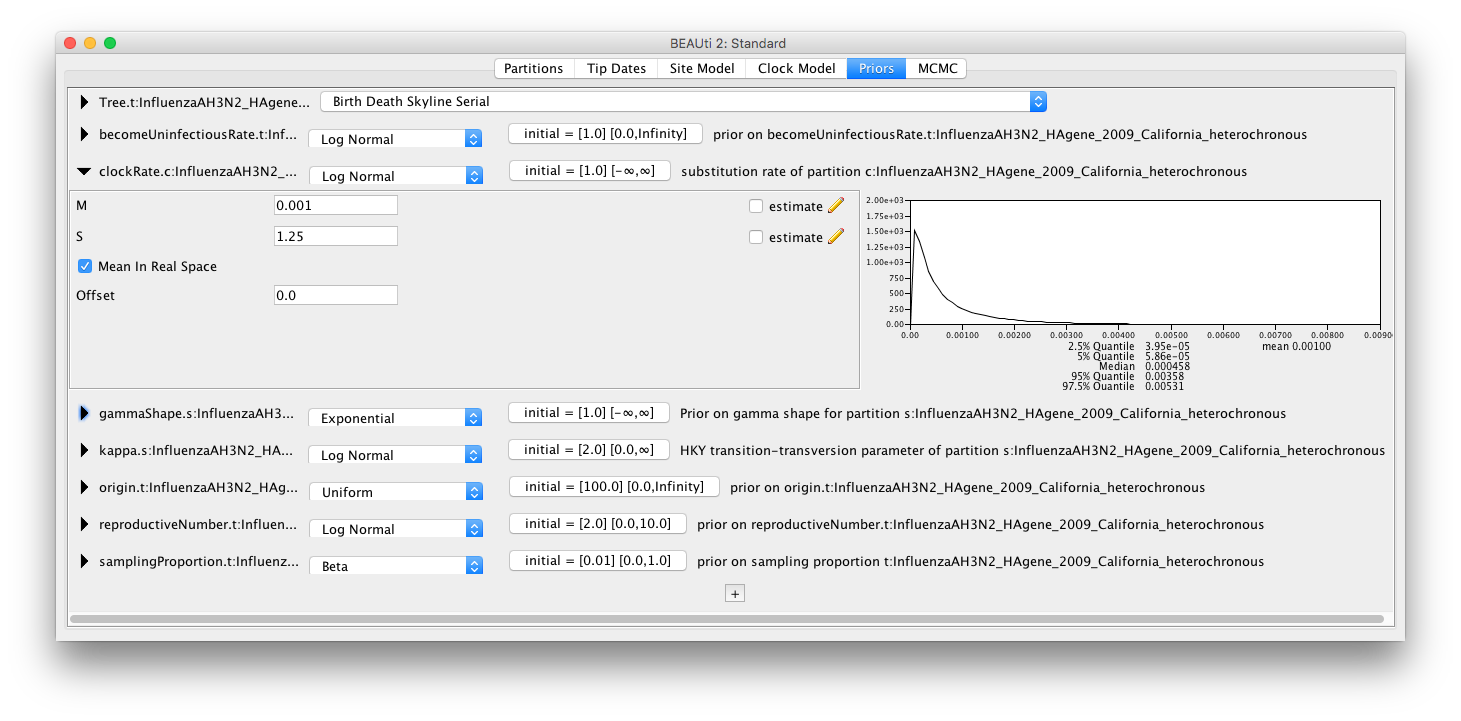
\includegraphics[max width=\textwidth, max height=0.9\textheight]{figures/beast2_prior_clockRate.png}
    \caption{Specifying the clock rate prior.}
    \label{clockRatePrior}
\end{figure}

We also need to estimate the Gamma shape parameter, which governs the
shape of the Gamma distribution of the rates across different sites. The
default setting of the Gamma shape parameter of \textbf{alpha=beta=1.0}
reflects our belief that on average, the rate scaler is equal to 1,
i.e.~on average all the sites mutate with the same substitution rate.
The distribution on the gamma shape parameter allows us to deviate from
this assumption. The default exponential distribution with \textbf{M}
(mean) of 1.0 and 95\%HPD of {[}0.0253,3.69{]} covers a wide range of
possible shape parameters. This looks fine for our analysis, and thus,
we leave the Gamma shape settings at its defaults (Figure
\ref{gammaShapeprior}).

\begin{figure}
    \centering
    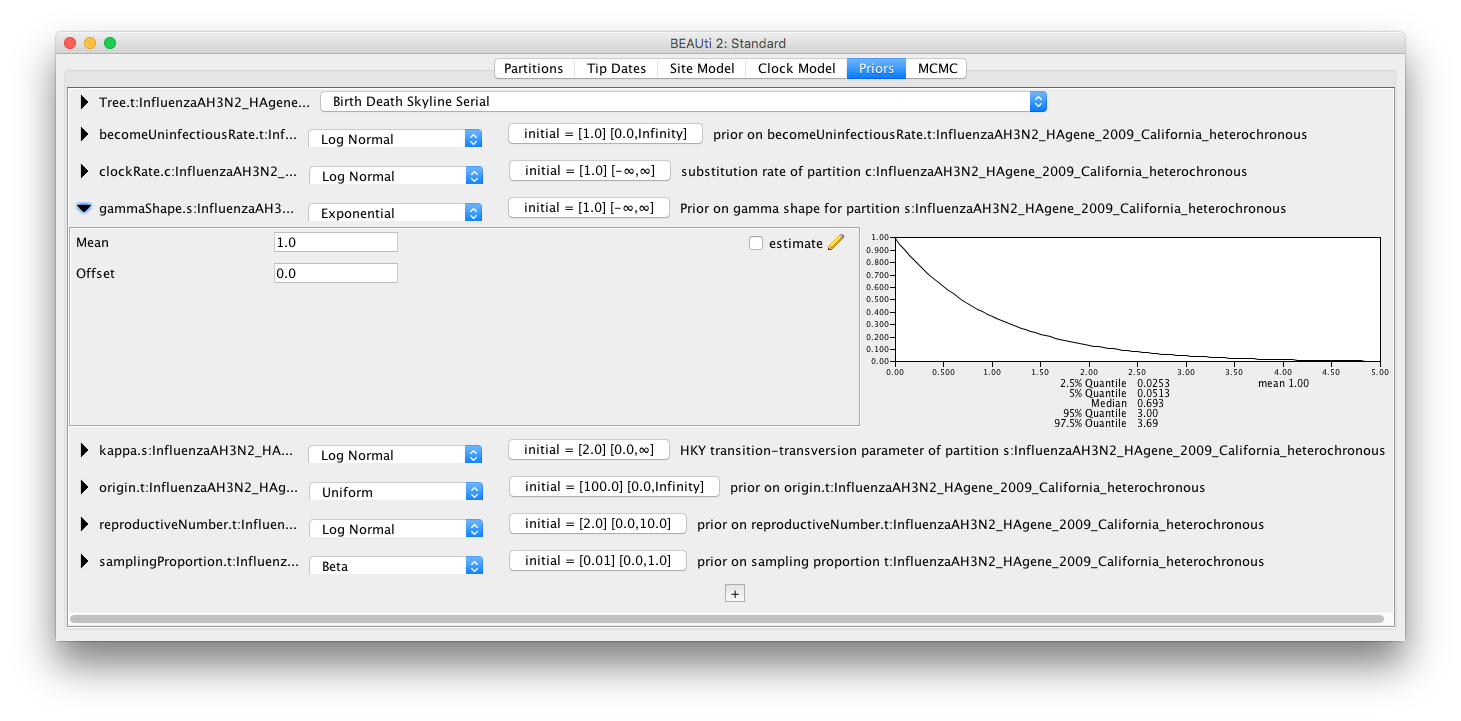
\includegraphics[max width=\textwidth, max height=0.9\textheight]{figures/beast2_prior_gammaShape.png}
    \caption{Specifying the gamma shape prior.}
    \label{gammaShapeprior}
\end{figure}

We do not have any prior information on transition-transversion ratio
besides the fact that it is a value usually larger than 1 (transitions
are more frequent than transversions). We therefore set a weakly
informative prior for this parameter. The default log normal prior
perfectly fits to these requirements and usually does not need to be
changed (Figure \ref{kappaPrior}).

\begin{figure}
    \centering
    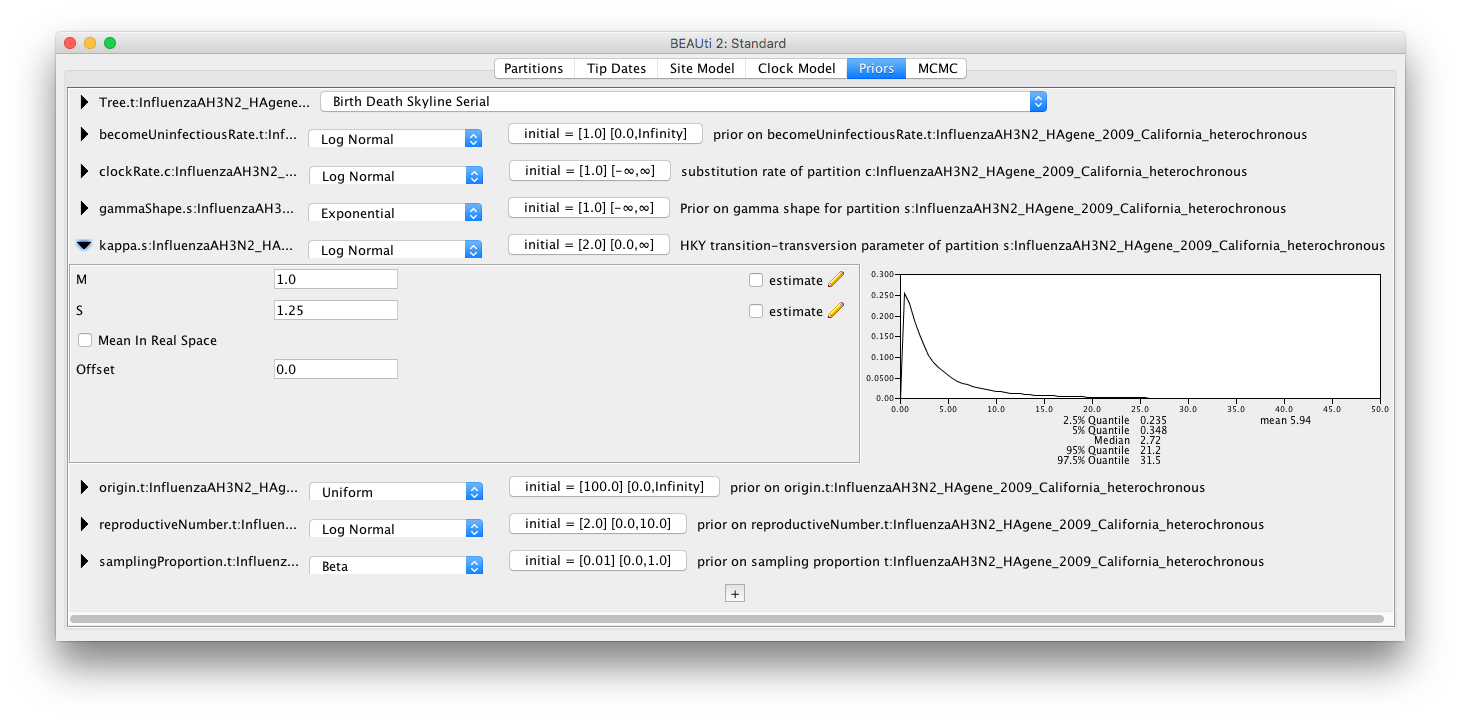
\includegraphics[max width=\textwidth, max height=0.9\textheight]{figures/beast2_prior_kappa.png}
    \caption{Specifying the kappa (transition/transversion ratio) prior.}
    \label{kappaPrior}
\end{figure}

For the next parameter, the origin of the epidemic, we ask ourselves
whether there is any reasonable expectation we might have in terms of
when the infection in California started, i.e.~what is the date when the
ancestor of all of the sequences first appeared.

\begin{framed}
\textbf{QUESTION: Do you have any feeling for what the origin
should/could be set to?}
\end{framed}

The data span a period of 3 months and come from a limited area; thus,
it would be unreasonable to assume that a single season flu epidemic
would last longer than a few months. The best guess for the origin
parameter prior we could make is therefore on the order of at least 3-4,
but probably no more than 6 months. We set the prior according to this
expectation.

\begin{framed}
Click on the arrow next to the \textbf{origin} and change the prior
distribution from \textbf{Uniform} to \textbf{Gamma} with \textbf{Alpha}
parameter set to 0.5 and \textbf{Beta} parameter set to 2.0 (Figure
\ref{originPrior}).
\end{framed}

\begin{figure}
    \centering
    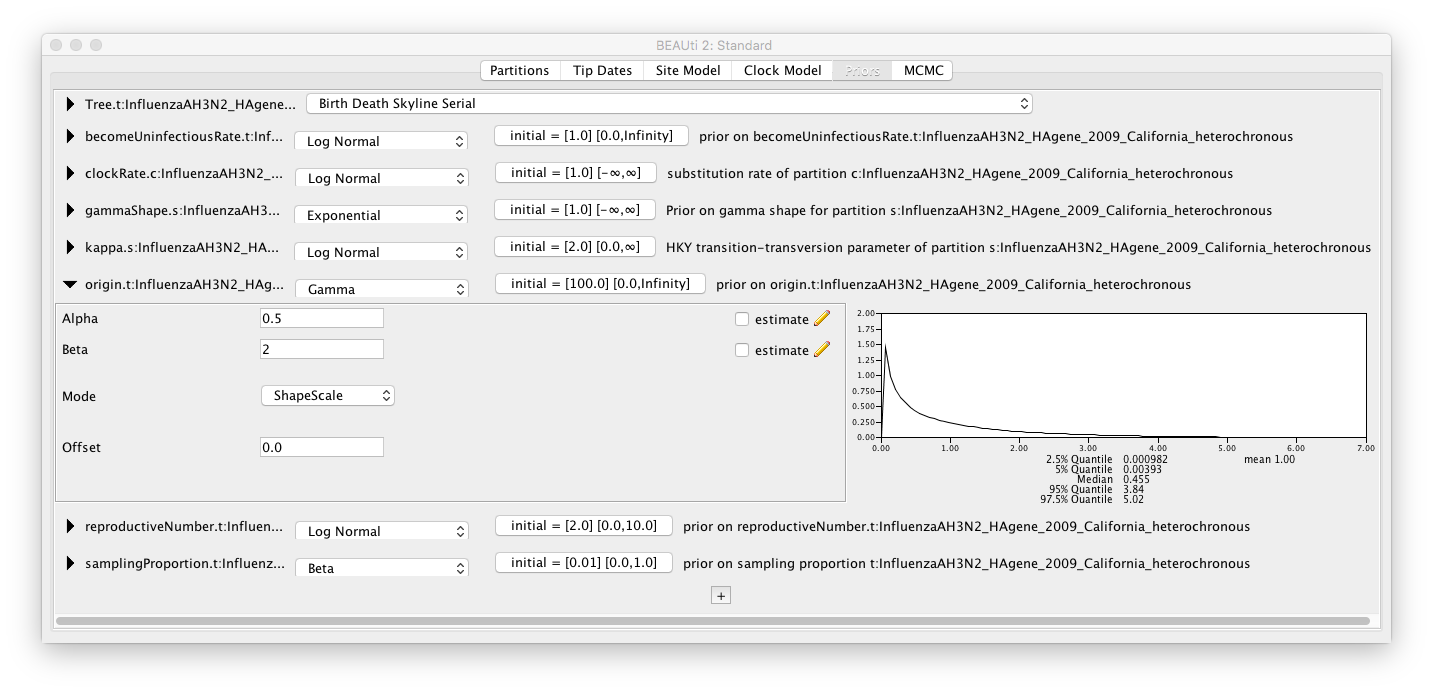
\includegraphics[max width=\textwidth, max height=0.9\textheight]{figures/beast2_prior_origin.png}
    \caption{Specifying the origin prior.}
    \label{originPrior}
\end{figure}

Lastly, for the sampling proportion, we know that we certainly did not
sample every single infected individual. Therefore, setting a prior
close to 1 would not be reasonable. Actually, it is more reasonable to
usually expect only a proportion of less than 0.1 of all flu cases to be
sampled. Here, we specify something on the order of 10$^{-3}$. The
default prior for the sampling proportion is a Beta distribution, which
is only defined between 0 and 1, making it a natural choice for
proportions. However, this is not the only prior that can be used, and
here we specify a log-normal distribution, while ensuring that an
appropriate upper limit is set, to prevent a sampling proportion higher
than 1, which is not defined.

\begin{framed}
Click on the arrow next to the \textbf{samplingProportion} and change
the distribution from \textbf{Beta} to \textbf{Log Normal}.

Next, change the value for the \textbf{M} (mean) to 0.001 and tick the
box \textbf{Mean In Real Space} (Figure \ref{samplingProportionPrior}).

Also, make sure that the \textbf{Lower} is set to 0.0 and the
\textbf{Upper} is set to 1.0.
\end{framed}

\begin{figure}
    \centering
    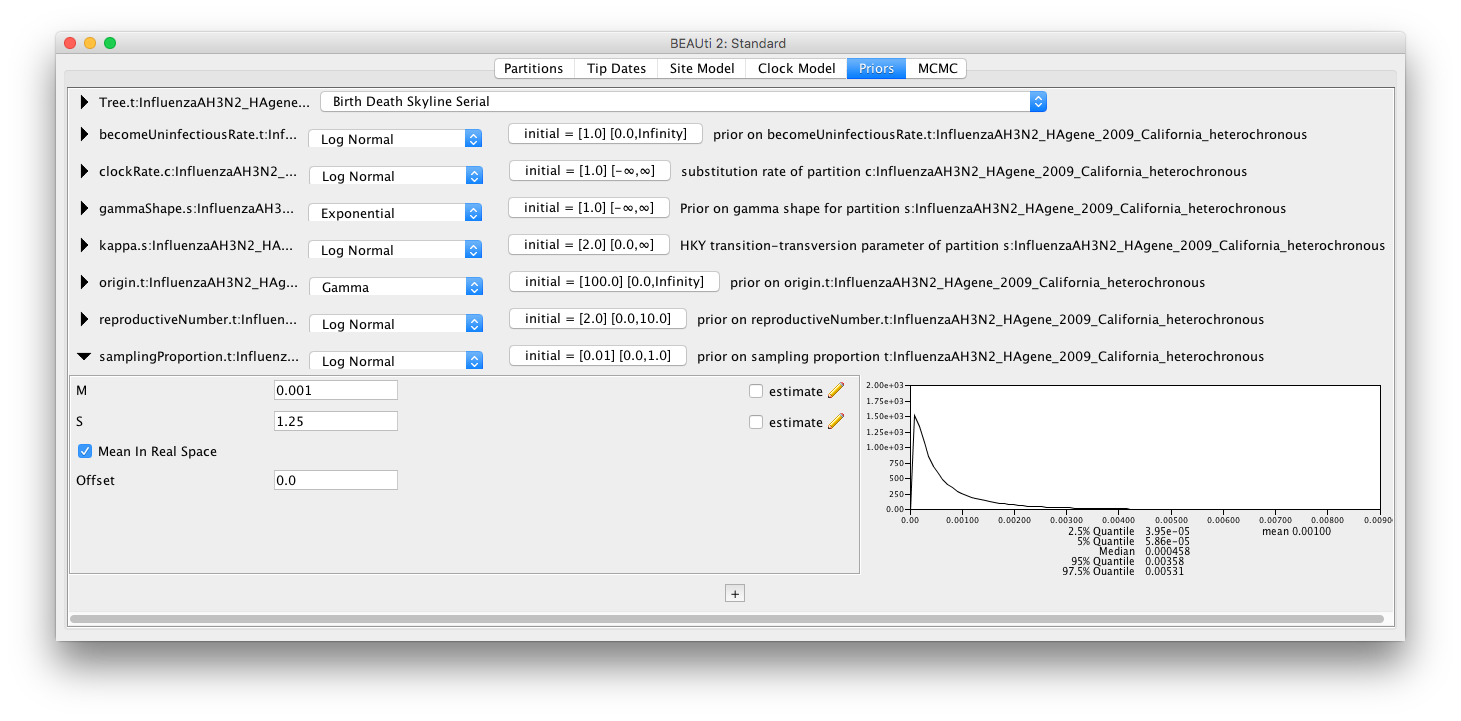
\includegraphics[max width=\textwidth, max height=0.9\textheight]{figures/beast2_prior_samplingProportion.png}
    \caption{Specifying the sampling proportion prior.}
    \label{samplingProportionPrior}
\end{figure}

\subsubsection{MCMC}\label{mcmc}

\begin{framed}
Navigate to the \textbf{MCMC} panel.
\end{framed}

We want to shorten the chain length, in order for it to run in a
reasonable time and we want to decrease the tree sampling frequency.

\begin{framed}
Change the \textbf{Chain Length} from 10'000'000 to 5'000'000.

Click on the arrow next to the \textbf{treelog} and set the \textbf{Log
Every} to 100'000 (Figure \ref{mcmc}).
\end{framed}

\begin{figure}
    \centering
    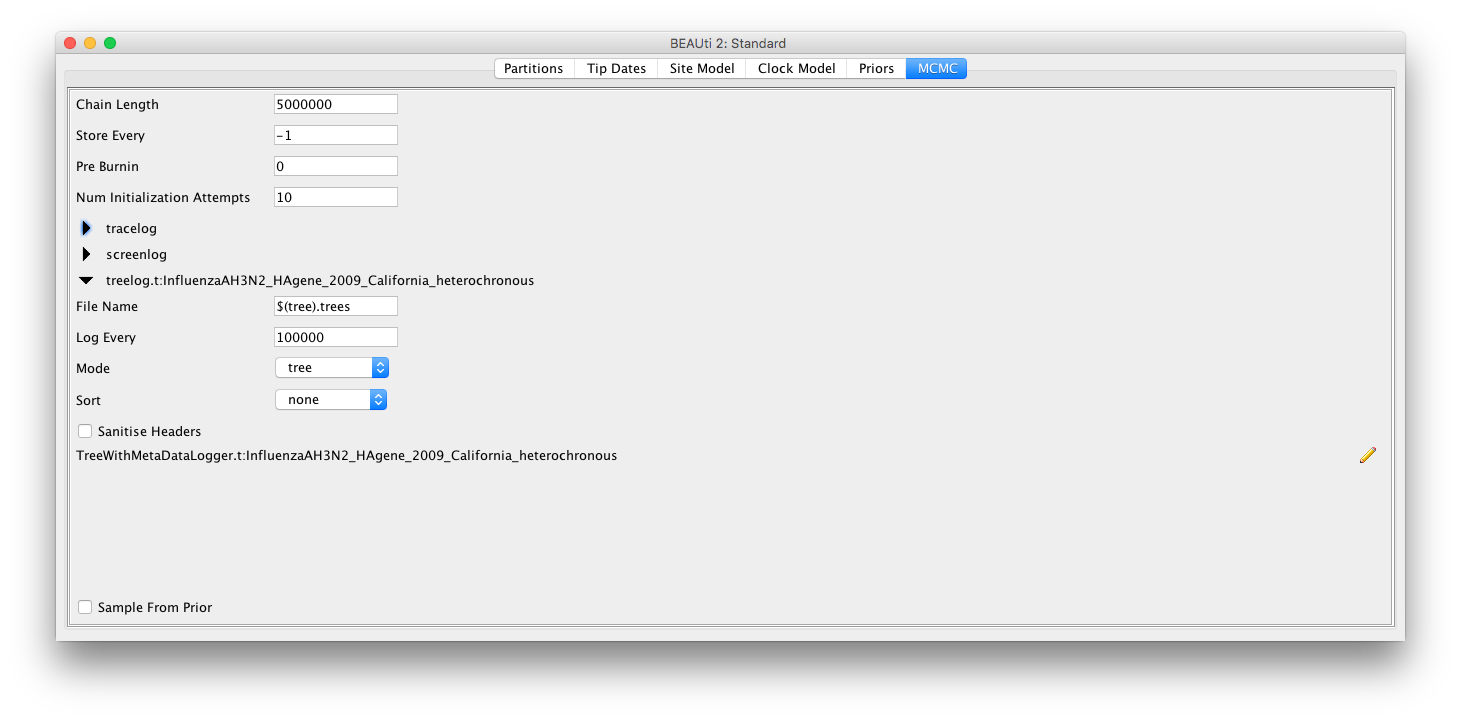
\includegraphics[max width=\textwidth, max height=0.9\textheight]{figures/beast2_mcmc.png}
    \caption{Specifying the MCMC properties.}
    \label{mcmc}
\end{figure}

Now, all the specifications are done. We want to save and run the XML.

\begin{framed}
Save the XML file as \lstinline!Heterochronous.xml!.
\end{framed}

\subsubsection{Running the analysis}\label{running-the-analysis}

\begin{framed}
Within BEAST, specify the file Heterochronous.xml.

If you have BEAGLE installed tick the box to \textbf{Use BEAGLE library
if available}, which will make the run faster.

Hit \textbf{Run} to start the analysis.
\end{framed}

The run should take about 15-20 minutes. While waiting for your results,
you can start preparing the XML file for the homochronous data.

\subsubsection{Analysing the results}\label{analysing-the-results}

\begin{framed}
Load the file into \textbf{Tracer} to check mixing and the parameter
estimates.
\end{framed}

\begin{figure}
    \centering
    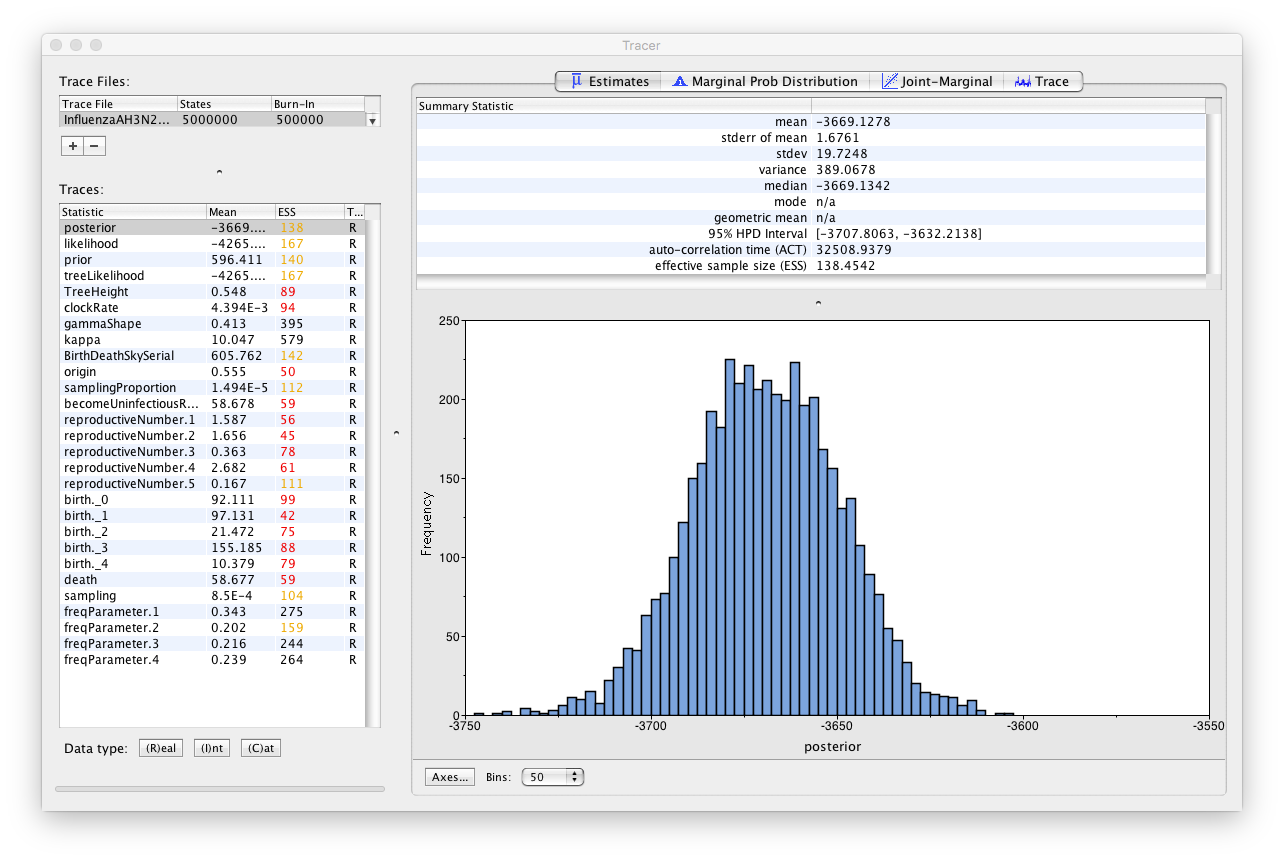
\includegraphics[max width=\textwidth, max height=0.9\textheight]{figures/tracer_short.png}
    \caption{Loading the log file into Tracer.}
    \label{tracershort}
\end{figure}

First thing you may notice is that most of the parameters do have low
ESS (effective sample size below 200) marked in red (Figure
\ref{tracershort}). This is because our chain did not run long enough.
However, the estimates we obtained with a chain of length 5'000'000 are
very similar to those obtained with a longer chain.

\begin{framed}
Click on \textbf{clockRate} and then click on \textbf{Trace} to examine
the trace of the parameter (Figure \ref{tracerclocktrace}).
\end{framed}

\begin{figure}
    \centering
    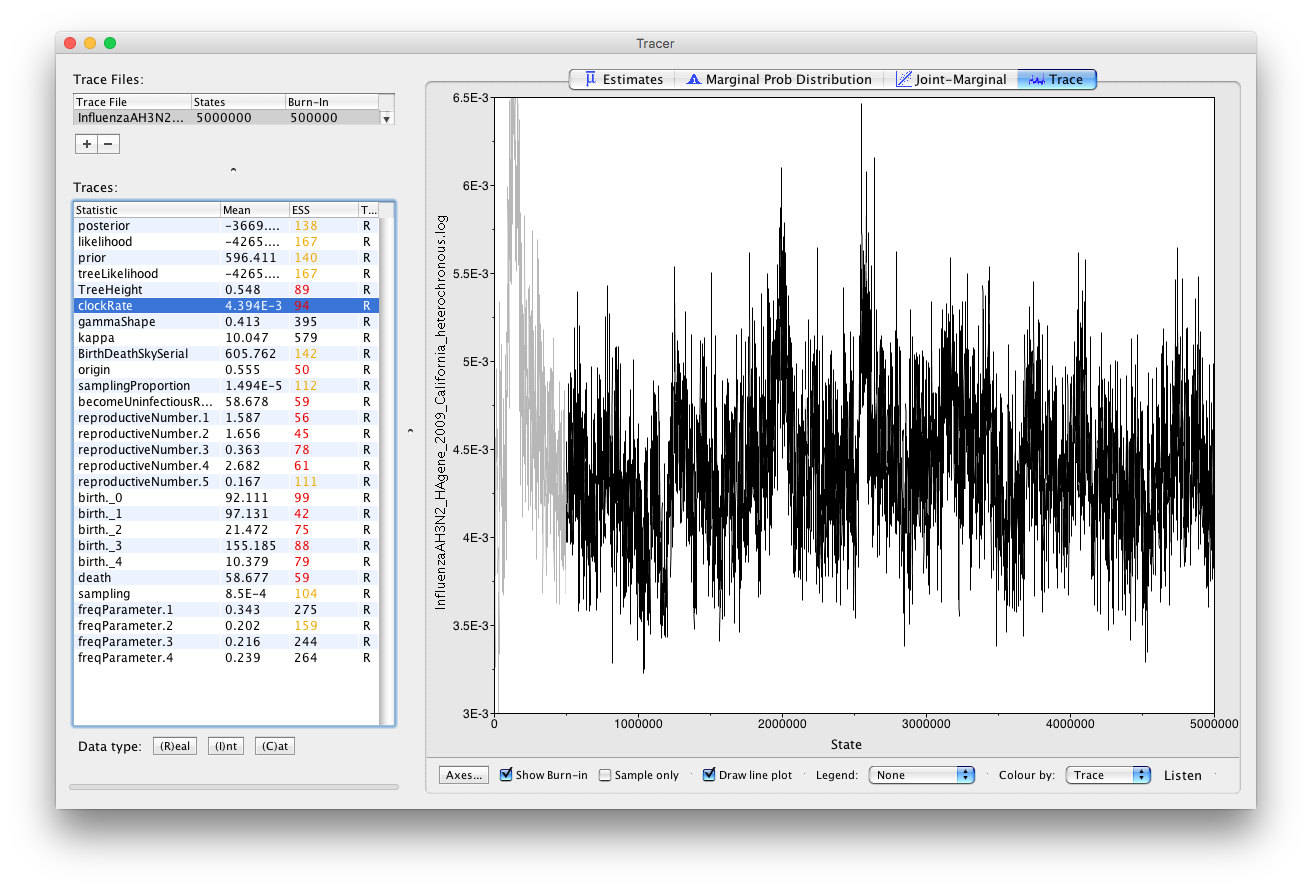
\includegraphics[max width=\textwidth, max height=0.9\textheight]{figures/tracer_clock_trace.png}
    \caption{The trace of the clock rate parameter.}
    \label{tracerclocktrace}
\end{figure}

Note that even though the parameter has a low ESS, the chain appears to
have passed the burn-in phase and seems to be sampling from across the
posterior without getting stuck in any local optima. This is not a proof
that the run is mixing well, however it gives us a good intuition that
the parameter will have a good ESS value if we run the chain for longer.
You should always examine the parameter traces to check convergence; a
high ESS value is not proof that a run has converged to the true
posterior.

If you like, you can compare your results with the example results we
obtained with identical settings and a chain of 30,000,000.

\begin{framed}
Load the file
\lstinline!InfluenzaAH3N2_HAgene_2009_California_heterochronous_30M.log!.

Do the parameter traces look better?

Examine the posterior estimates for the \textbf{becomeUninfectiousRate},
\textbf{samplingProportion} and \textbf{clockRate} in Tracer. Do the
estimates look realistic? Are they different from the priors we set and
if so, how?
\end{framed}

The estimated posterior distribution for the
\textbf{becomeUninfectiousRate} has a median of 58.376 and a 95\% HPD
between 43.2389 and 77.6039 (Figure \ref{tracerdelta}). This is
between$ \approx $ 4.7 and 8.44 days, thus, roughly one
week. This is a lot more specific than the prior we set, which allowed
for a much longer infectious period. The estimates also agree with what
we know about Influenza A. In this case there was enough information in
the sequencing data to estimate a more specific becoming uninfectious
rate. If we had relied more on our prior knowledge we could have set a
tighter prior on the \textbf{becomeUninfectiousRate} parameter, which
may have helped the run to converge faster, by preventing it from
sampling unrealistic parameter values. However, if you are unsure about
a parameter it is always better to set more diffuse priors.

\begin{figure}
    \centering
    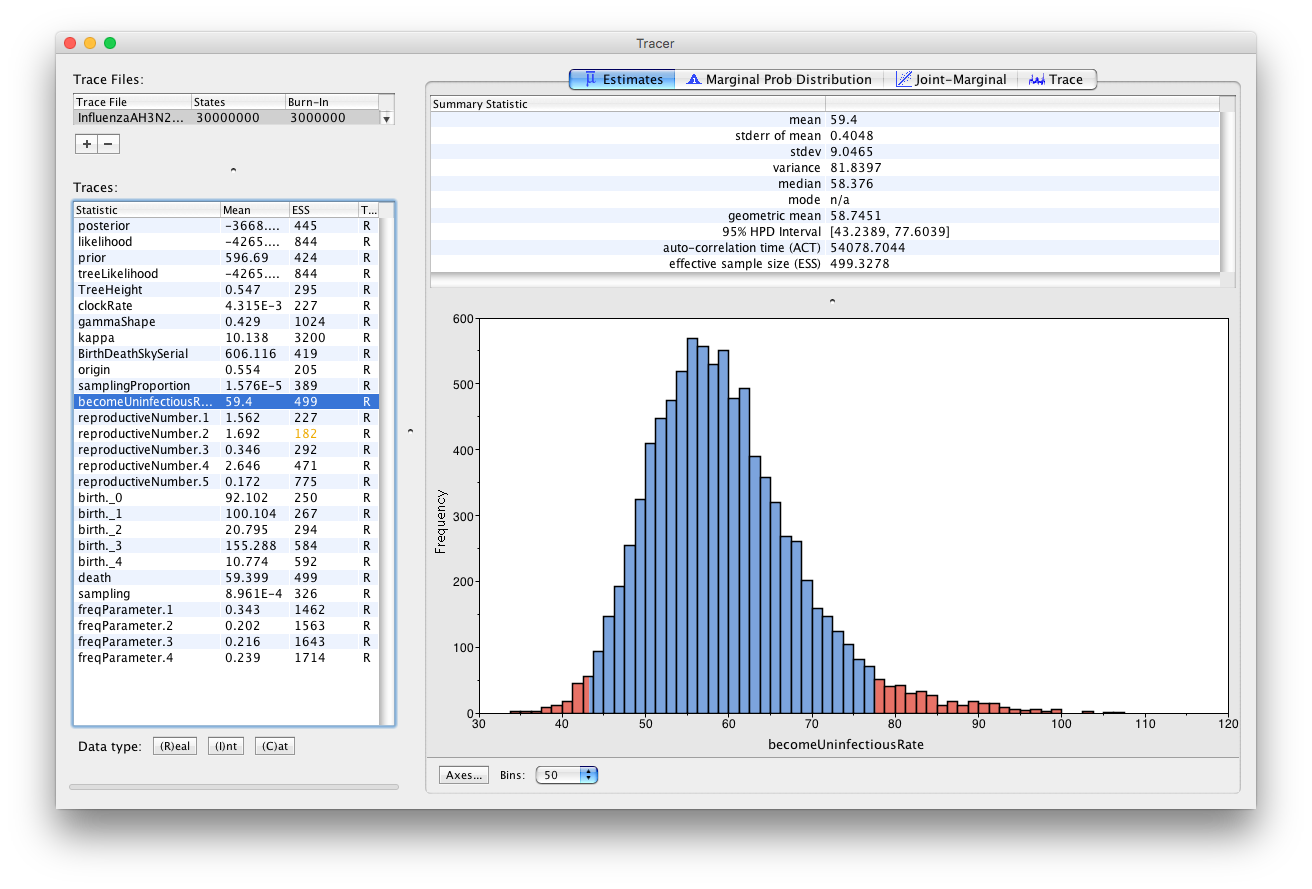
\includegraphics[max width=\textwidth, max height=0.9\textheight]{figures/tracer_becomeUninfectiousRate.png}
    \caption{Estimated posterior distribution for the becoming uninfectious rate.}
    \label{tracerdelta}
\end{figure}

We see that the sampling proportion (Figure \ref{tracersampling}) is
estimated to be below $ 5 \times $ 10$^{-5}$. This a lot
lower than the mean we set for the prior on the sampling proportion
(0.001). Therefore our prior estimate of the sampling proportion was
much too high. Consequently, we see that the number of cases is also
much higher than we initially thought. We assumed that there are around
1,000 cases when we set the prior, however our posterior indicates that
the epidemic has on the order of tens of thousands of cases.

\begin{figure}
    \centering
    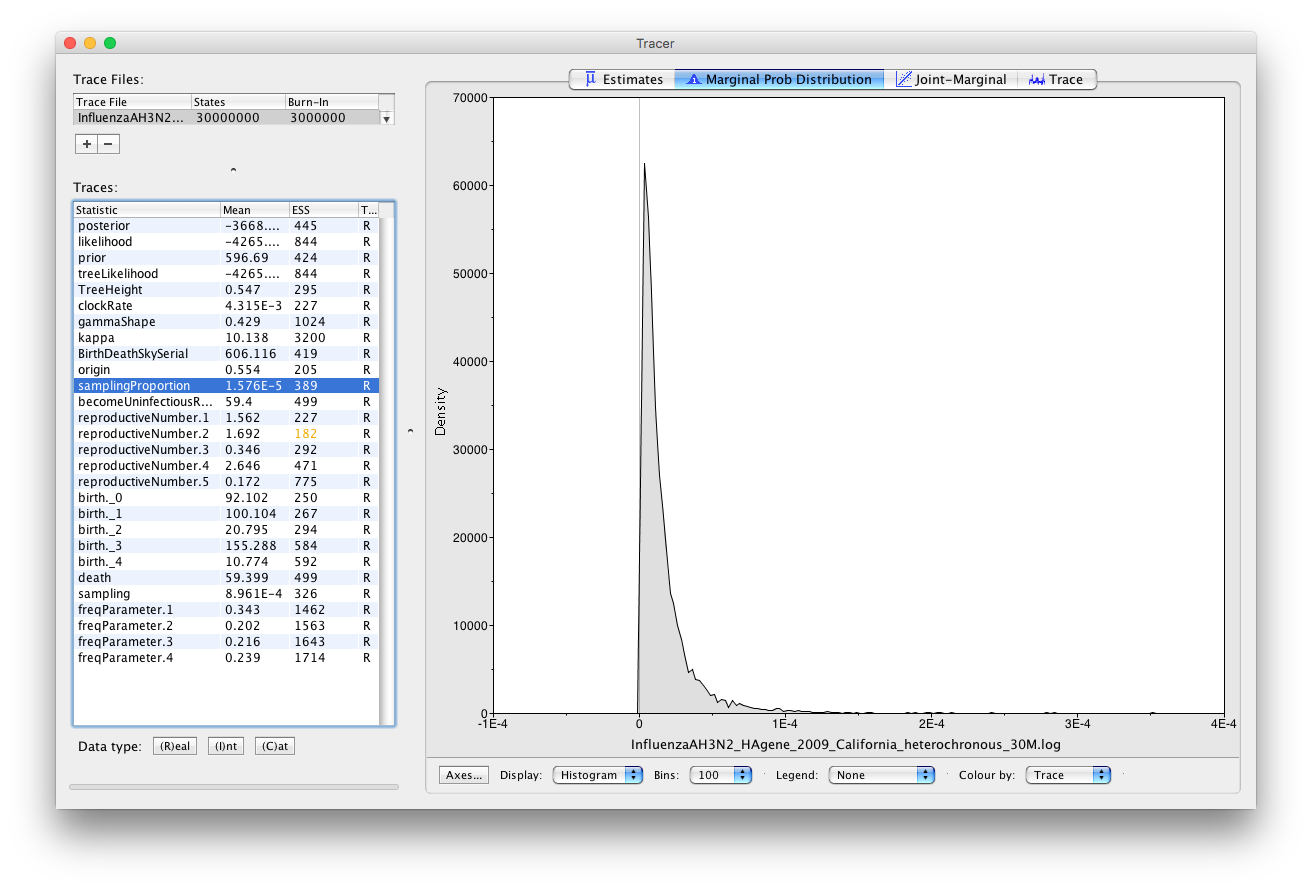
\includegraphics[max width=\textwidth, max height=0.9\textheight]{figures/tracer_samplingProportion.png}
    \caption{Estimated posterior distribution for the sampling proportion.}
    \label{tracersampling}
\end{figure}

Looking at the clock rate estimates (Figure \ref{tracerclockRate}) we
that they are about 2 to 3 times faster than the usual substitution rate
for human influenza A \citep{jenkins2002}. This is not a cause for
concern and is actually a well-documented phenomenon. When viral samples
are collected over a short time period the clock rate is often
overestimated. The exact cause of the bias is not known, but it is
suspected that incomplete purifying selection plays a role. What is
important to keep in mind is that this is does not mean that the virus
is mutating or evolving faster than usual. When samples are collected
over a longer time period the estimated clock rate slows down and
eventually reaches the long-term substitution rate.

\begin{figure}
    \centering
    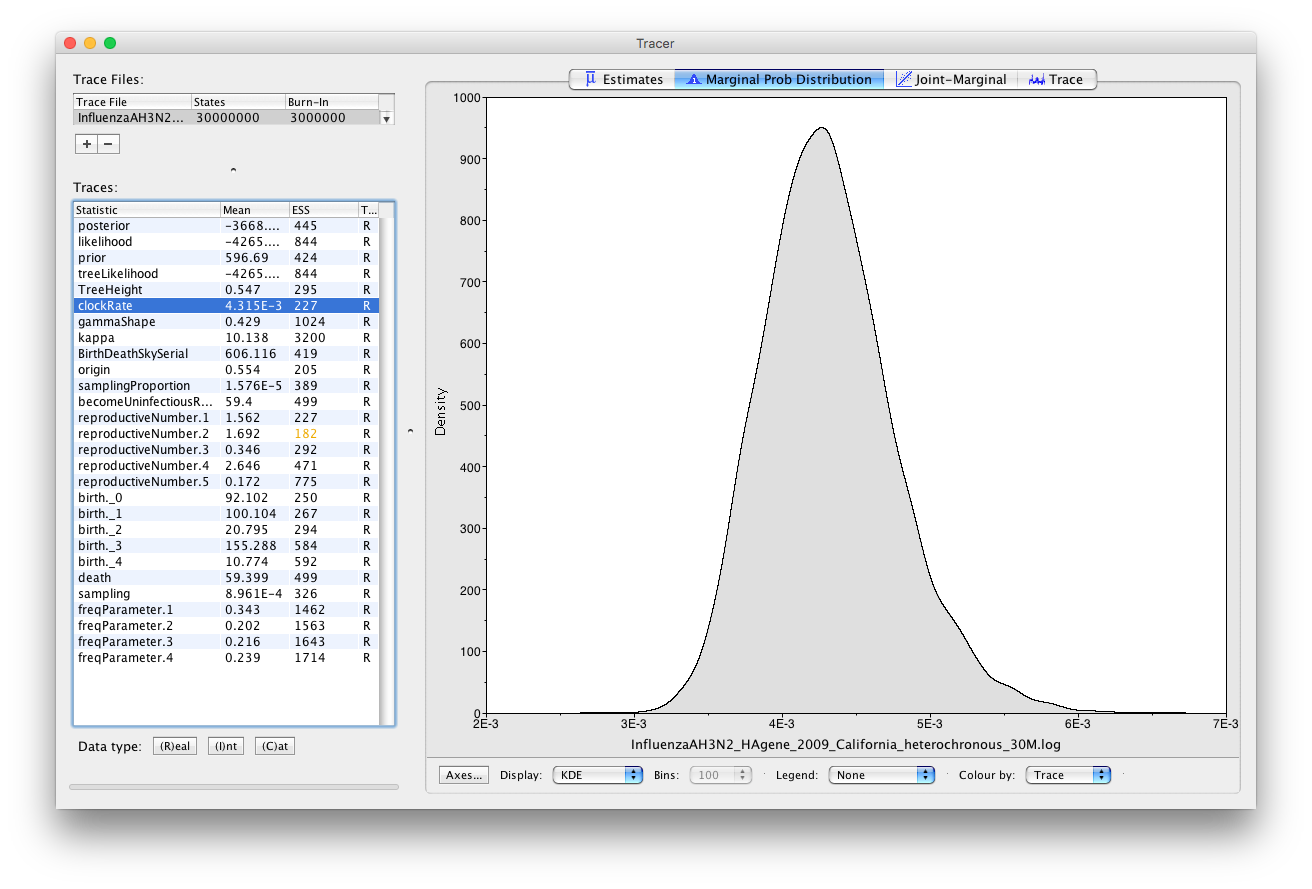
\includegraphics[max width=\textwidth, max height=0.9\textheight]{figures/tracer_clockRate.png}
    \caption{Estimated posterior distribution for the clock rate.}
    \label{tracerclockRate}
\end{figure}

\section{Practical: H3N2 flu dynamics - homochronous
data}\label{practical-h3n2-flu-dynamics---homochronous-data}

We could also use the homochronous data to investigate the dynamics of
the H3N2 spread in California in 2009. We use the 29 sequences from
April 28, 2009 to investigate whether this is possible.

Follow the same procedure as for the heterochronous sampling. Now,
however, use the alignment file called
\lstinline!InfluenzaAH3N2_HAgene_2009_California_homochronous.nexus! and
use the \textbf{Birth Death Skyline Contemporary} model.

Note that for the \textbf{Birth Death Skyline Contemporary} model the
sampling proportion is called \textbf{rho}, and refers only to the
proportion of infected individuals sampled at the present time. This is
to distinguish it from the sampling proportion in the \textbf{Birth
Death Skyline Serial} model, which refers to the proportion of
individuals sampled through time.

\begin{figure}
    \centering
    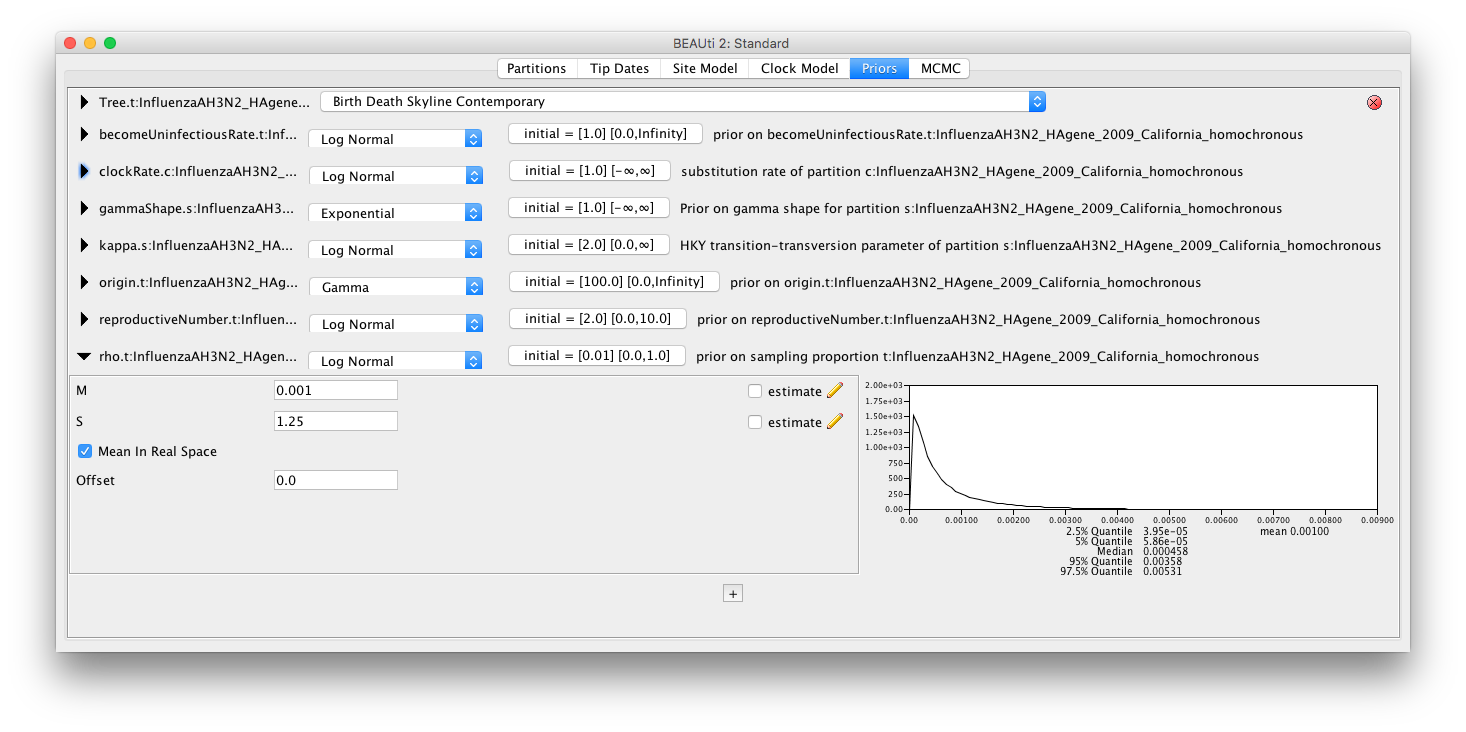
\includegraphics[max width=\textwidth, max height=0.9\textheight]{figures/beast2_prior_rho.png}
    \caption{Specifying the sampling proportion prior for homochronous data.}
    \label{rho}
\end{figure}

\subsection{Estimating the substitution rate from homochronous
data}\label{estimating-the-substitution-rate-from-homochronous-data}

\begin{framed}
After the run is finished, load the log file into Tracer.

Examine the traces of the parameters. Do you think running the analysis
for longer will lead to the run mixing well?
\end{framed}

Most of the parameters again have ESS values below 200, however in this
case the ESS values are lower than for heterochronous data and it is not
clear that running the analysis for longer will lead to mixing. Indeed,
while running the analysis for longer increases increases the ESS values
for some parameters, however they remain low for some parameters, in
particular the \textbf{origin}, \textbf{TreeHeight} (tMRCA) and
\textbf{clockRate}. Low ESS values for these parameters in turn
translate into low ESS values for the tree prior
(\textbf{BirthDeathSkyContemporary}), prior and posterior.

\begin{figure}
    \centering
    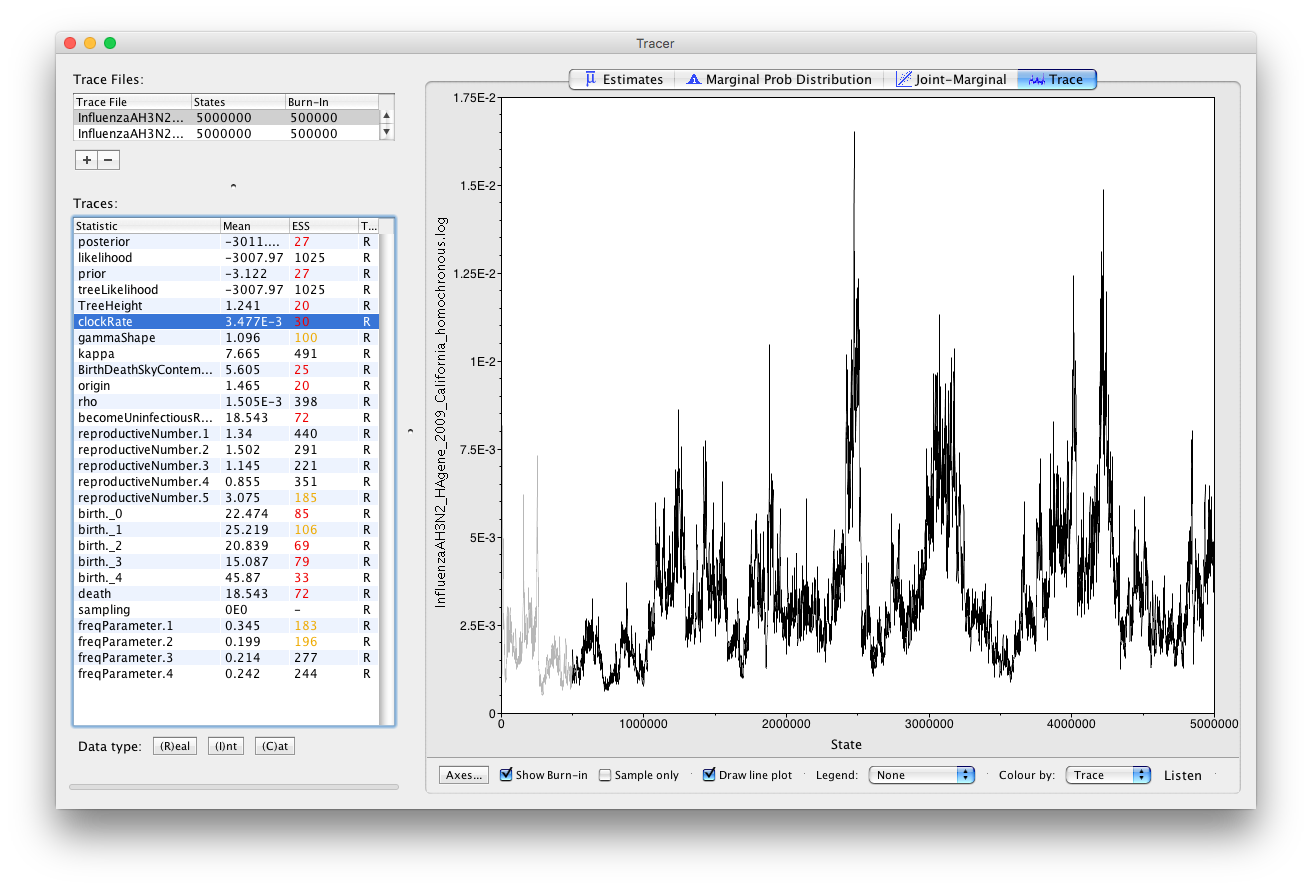
\includegraphics[max width=\textwidth, max height=0.9\textheight]{figures/tracer_clockTrace2.png}
    \caption{The trace of the clock rate parameter.}
    \label{tracerclocktrace2}
\end{figure}

Now, check the clock rate and the tree height parameters.

\begin{framed}
\textbf{QUESTION: Do you think that homochronous samples allow for good
substitution rate estimation?}

\textbf{If yes, how would you know?}

\textbf{If not, how can you see that and where do you think might the
problem be? Can we address this problem in our analysis?}
\end{framed}

Notice the values of the substitution rate estimates. From literature,
one can read that influenza's HA gene has a substitution rate of about
10$^{-3}$ substitutions per site per year \citep{jenkins2002}. Our
estimate of the clock rate is of the same order as this value, but has a
very large confidence interval. Notice also, that the confidence
interval of the tree height is very large {[}0.1305,2.7393{]}.

Another way to see that the homochronous sampling does not allow for the
estimation of the clock rate is to observe a very strong negative
correlation of the clock rate with the tree height.

\begin{framed}
In \textbf{Tracer} click on the \textbf{Joint Marginal} panel, select
the \textbf{TreeHeight} and the \textbf{clockRate} simultaneously, and
uncheck the \textbf{Sample only} box below the graphics (Figure
\ref{clockRatetreeHeightCorrelation}).
\end{framed}

\begin{figure}
    \centering
    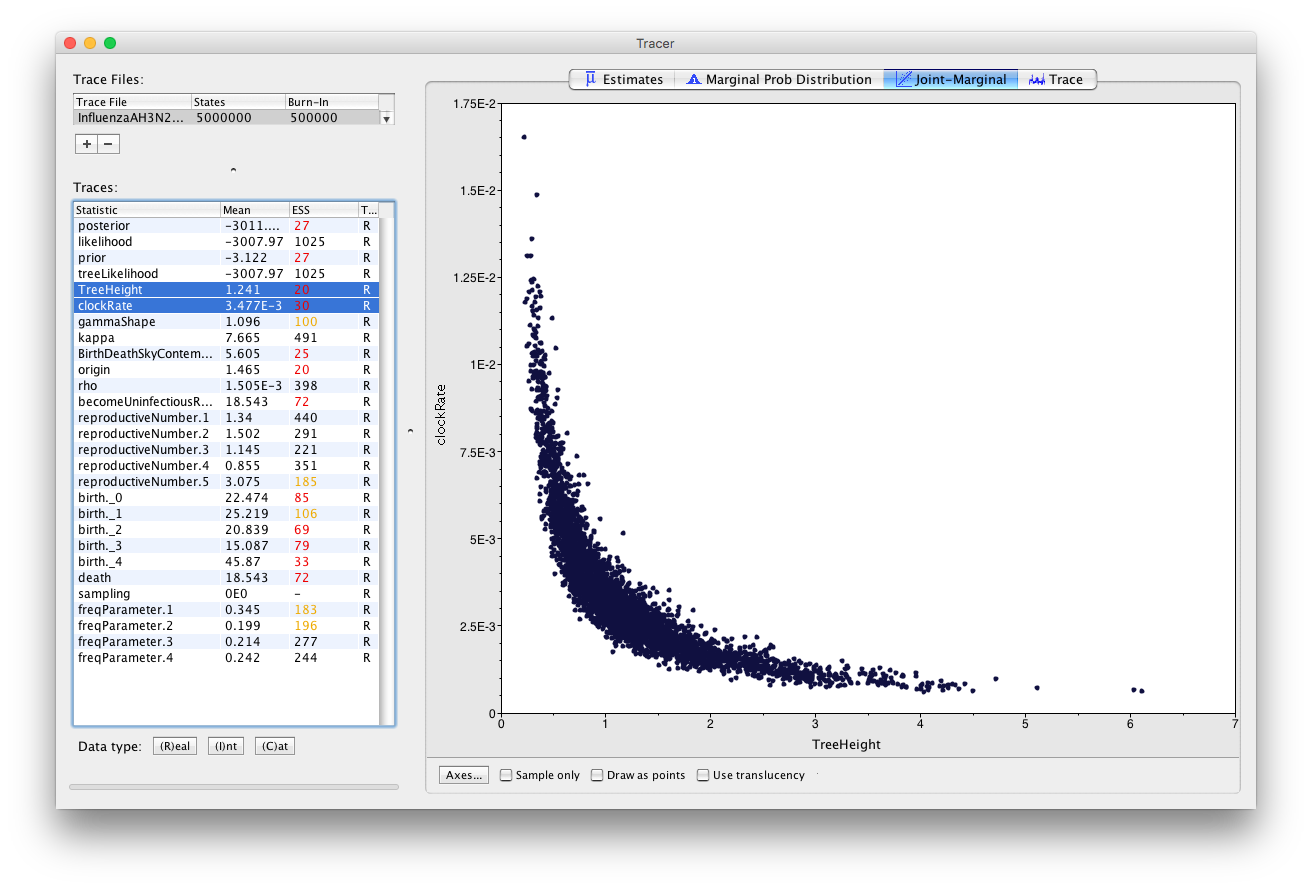
\includegraphics[max width=\textwidth, max height=0.9\textheight]{figures/tracer_homochronous_treeHeightclockRatecorrelation.png}
    \caption{Clock rate and tree height correlation in homochronous data.}
    \label{clockRatetreeHeightCorrelation}
\end{figure}

The correlation between the tree height and the clock rate is obvious:
the taller the tree, the slower the clock. One way to solve this problem
is to break this correlation by setting a strong prior on one of the two
parameters. We describe how to set a prior on the tree height in the
section below.

\subsubsection{Creating Taxon Sets}\label{creating-taxon-sets}

We will use the results from the heterochronous data, to find out what a
good estimate for the tree height of these homochronous samples is. For
this aim, we first create an MCC (maximum clade credibility) tree in the
\textbf{TreeAnnotator} and then check with \textbf{FigTree} what the
estimate of the tMRCA (time to the most recent common ancestor) of the
samples from April 28, 2009 is.

Note, however, that we do this for illustration purposes only. In good
practice, one should avoid re-using the data or using the results of an
analyses to inform any further analyses containing the same data. Let's
pretend therefore that the heterochronous dataset is an independent
dataset from the homochronous one.

\begin{framed}
Open the \textbf{TreeAnnotator} and set \textbf{Burnin percentage} to
10, \textbf{Posterior probability limit} to 0.5. Leave the other options
unchanged.

Set the \textbf{Input Tree File} to
\lstinline!InfluenzaAH3N2_HAgene_2009_California_heterochronous.trees!
and the \textbf{Output File} to
\lstinline!InfluenzaAH3N2_HAgene_2009_California_heterochronous.tree!.
(Figure \ref{treeAnnotator})
\end{framed}

\begin{figure}
    \centering
    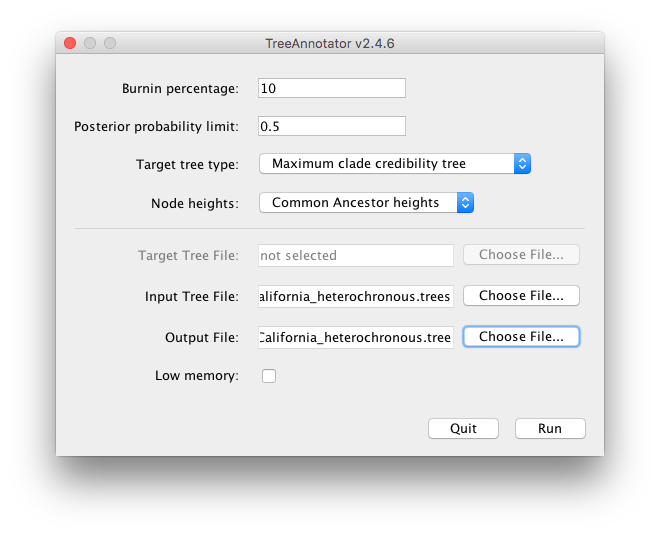
\includegraphics[width=0.500000\textwidth]{figures/treeAnnotator.png}
    \caption{Creating the MCC tree.}
    \label{treeAnnotator}
\end{figure}

How can we find out what the tMRCA of our homochronous data may be? The
best may be to have a look at the estimates of the heterochronous data
in the \textbf{FigTree}.

\begin{framed}
Now open \textbf{FigTree} and load
\lstinline!InfluenzaAH3N2_HAgene_2009_California_heterochronous.tree!.

In the upper right corner, next to the magnifier glass sign, type
\textbf{2009/04/28} to highlight all the sequences from April 28, 2009.
(Figure \ref{tMRCAmedian})
\end{framed}

\begin{figure}
    \centering
    \includegraphics[max width=\textwidth, max height=0.9\textheight]{figures/FigTree_tMRCA_median.png}
    \caption{Displaying median estimates of the node height in the MCC tree.}
    \label{tMRCAmedian}
\end{figure}

\begin{framed}
Tick the \textbf{Node Labels} in the left menu, and click the arrow next
to it to open the full options. Change the \textbf{Display} from
\textbf{age} to \textbf{height\_median} (Figure \ref{tMRCAmedian}) and
then to **height\_95\%\_HPD** (Figure \ref{tMRCA95HPD}).
\end{framed}

\begin{figure}
    \centering
    \includegraphics[max width=\textwidth, max height=0.9\textheight]{figures/FigTree_tMRCA_HPD.png}
    \caption{Displaying 95\% HPD estimates of the node height in the MCC tree.}
    \label{tMRCA95HPD}
\end{figure}

Notice, that since we are using only a subset of all the heterochronous
sequences, we are interested in the tMRCA of the samples from April 28,
2009 which may not coincide with the tree height of all the
heterochronous data. These samples are spread around over all the clades
in the tree, and the most recent common ancestor of all of them turns
out to be the root of the MCC tree of the heterochronous samples. We
therefore want to set the tMRCA prior of the tree formed by the
homochronous sequences to be peaked around the median value of the MCC
tree height, which is 0.5488 and we want 95\% of the density of the
prior distribution to be between 0.5343-0.5603.

\begin{framed}
Open BEAUti, load the homochronous data and use the same settings as for
the \lstinline!Homochronous.xml! file.

Create a new taxon set for root node by clicking the \textbf{+} at the
bottom of the parameter list in the \textbf{Priors} window. Select
\textbf{MRCA prior} in the dropdown menu and press \textbf{OK}. This
will reveal the \textbf{Taxon set editor}.

Change the \textbf{Taxon set} label to \textbf{allseq}.

Select the sequences belonging to this clade, i.e.~all the tips, and
move them from the left column to the right column using the
\textbf{\textgreater{} \textgreater{}} button and click \textbf{OK}.
(Figure \ref{tMRCAPrior})
\end{framed}

\begin{figure}
    \centering
    \includegraphics[width=0.750000\textwidth]{figures/beast2_homochronous_tMRCA.png}
    \caption{Specifying the root height prior.}
    \label{tMRCAPrior}
\end{figure}

The prior that we are specifying is the date (not the height) of the
tMRCA of all the samples in our dataset. Thus, we need to recalculate
the date from the tMRCA height estimates that we obtained above. All the
tips are sampled at the date $ \approx $ 2009.3233. The
median date of the MRCA should therefore be calculated as follows
2009.3233 - 0.5488 = 2008.7745 and the 95\% HPD should be
{[}2009.3233-0.5603, 2009.3233-0.5343{]}={[}2008.763,2008.789{]}.

\begin{framed}
Back in the \textbf{Priors} window, check the box labeled
\textbf{monophyletic} for the \textbf{allseq.prior}.

Click on the arrow next to the \textbf{allseq.prior}. Change the prior
distribution on the time of the MRCA of selected sequences from
\textbf{{[}none{]}} to \textbf{Laplace Distribution} and set the
\textbf{Mu} to 2008.7745 and the \textbf{Scale} to 0.01 (Figure
\ref{tMRCAPrior2}).

You can check that these settings correspond to the height of tMRCA from
the MCC tree by setting \textbf{Mu} to 0.5488 and observing the
distribution to the right. When you are done, do not forget to set
\textbf{Mu} back to 2008.7745.
\end{framed}

\begin{figure}
    \centering
    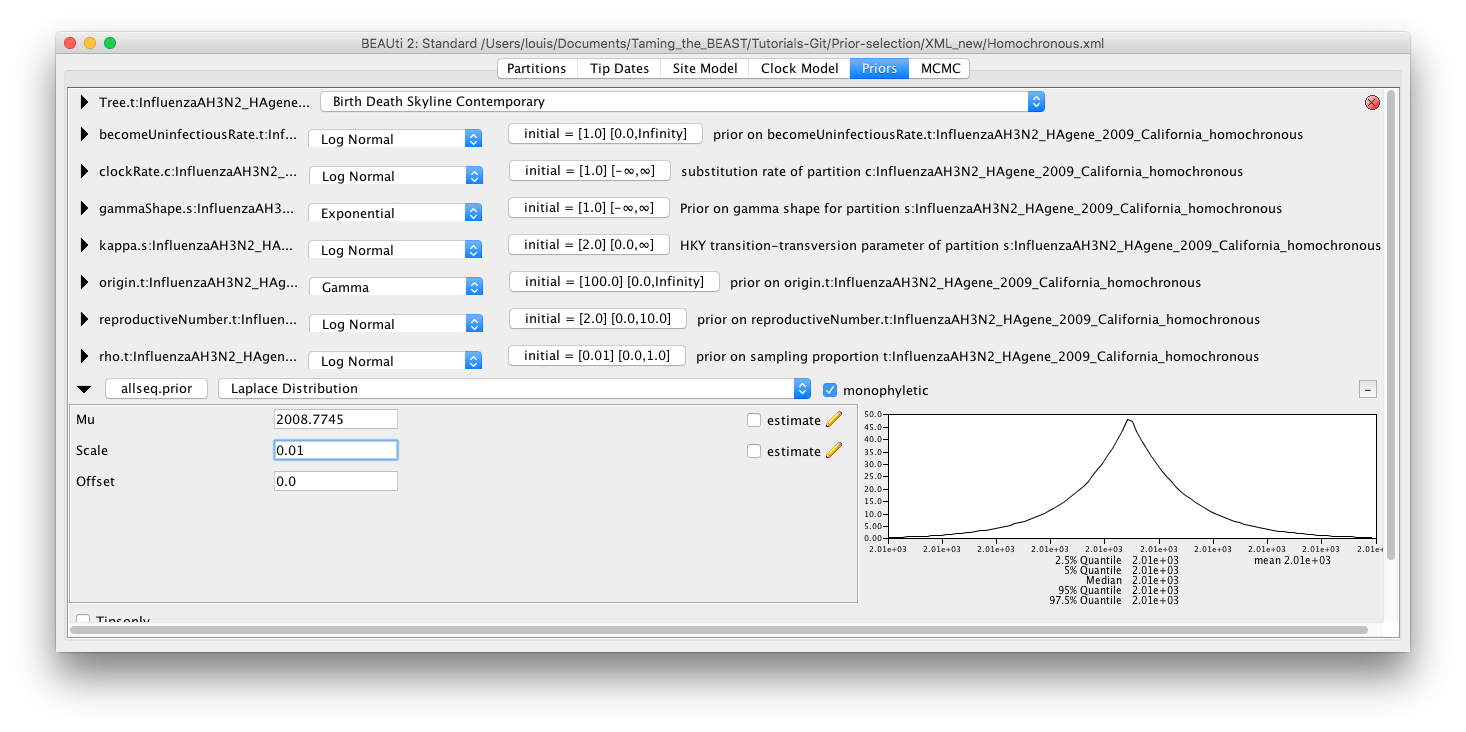
\includegraphics[max width=\textwidth, max height=0.9\textheight]{figures/beast2_homochronous_tMRCA_prior.png}
    \caption{Specifying the root height prior.}
    \label{tMRCAPrior2}
\end{figure}

We also need to change the names of the output files so that we do not
overwrite the results of the previous analyses.

\begin{framed}
In the \textbf{MCMC} window, click on the arrow next to the
\textbf{tracelog} and change the \textbf{File Name} to
\lstinline!InfluenzaAH3N2_HAgene_2009_California_homochronous_tMRCA.log!.

Then, click on the arrow next to the \textbf{treelog} and add
\lstinline!_tMRCA! between \lstinline!$(tree)! and \lstinline!.trees! in
the \textbf{File Name} field.
\end{framed}

Save the XML file as \lstinline!Homochronous_tMRCA.xml! and run the
analysis and compare to the original analysis of the homochronous data.
Are the substitution rate estimates more precise now?

\section{Comparison between runs}\label{comparison-between-runs}

\begin{framed}
Load the log files for all three analyses into Tracer.

Select \textbf{clockRate} and then press \lstinline!shift! to select all
three trace files.

Click on \textbf{Marginal Prob Distribution}, selected
\textbf{Top-Right} for the legend and colour by \textbf{Trace File}.

How do the estimates for the three analyses compare to each other?

Now repeat for the \textbf{TreeHeight}.
\end{framed}

\begin{figure}
    \centering
    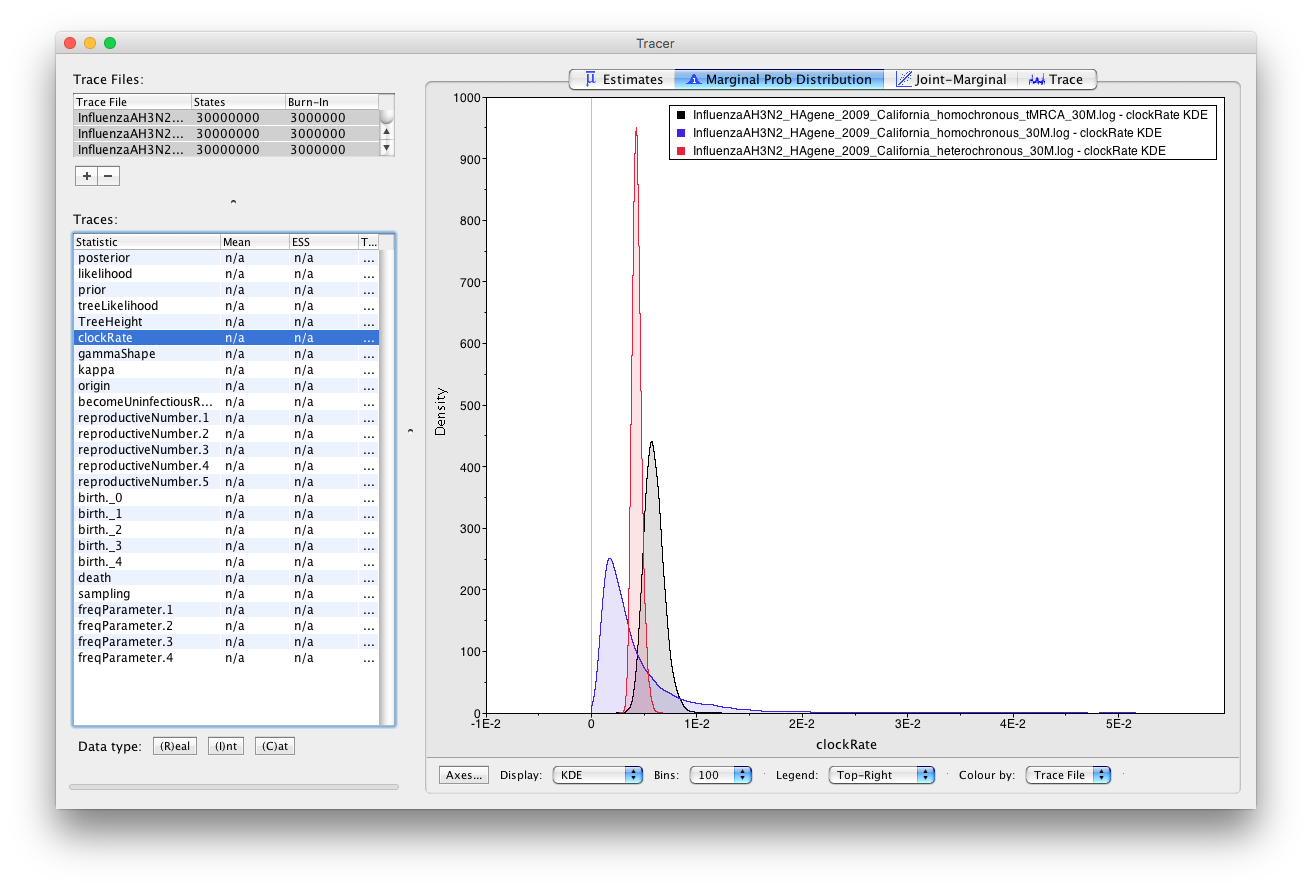
\includegraphics[max width=\textwidth, max height=0.9\textheight]{figures/tracer_clockcomparison.png}
    \caption{Comparing the marginal posteriors of the clock rate.}
    \label{tracerclockcompare}
\end{figure}

\begin{figure}
    \centering
    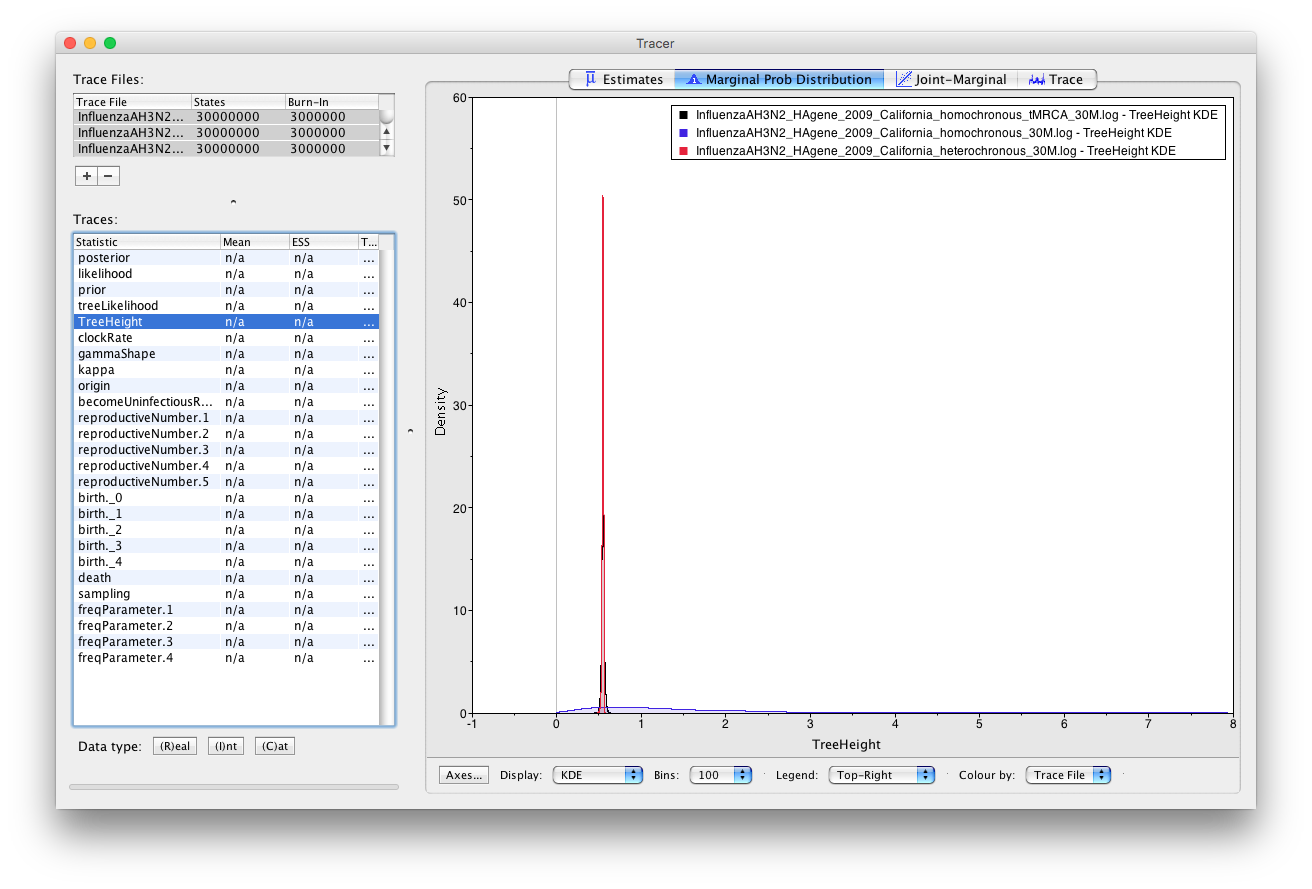
\includegraphics[max width=\textwidth, max height=0.9\textheight]{figures/tracer_tmrcacomparison.png}
    \caption{Comparing the marginal posteriors of the tMRCA.}
    \label{tracertmrcacompare}
\end{figure}

We see that the heterochronous analysis has the tightest posterior
estimates for the clock rate. Hence, it is clear that this dataset
contains the most information about the clock rate. This is obvious,
since this dataset not only contains sequences sampled across time, but
it also contains many more sequences than the homochronous dataset. The
marginal posterior for the clock rate estimated from homochronous data
with a prior on the tMRCA approaches this distribution, however it is
still more diffuse. On the other hand, the clock rate estimates made on
the homochronous data without a tMRCA prior are very diffuse. It is
important to note that these estimates are \textbf{not} wrong, but
simply indicates that there is a lot of uncertainty in the data.
Importantly, the true clock rate still falls within the 95\% HPD of the
estimated clock rate from homochronous data. If this were not the case
then the estimates would be wrong. Thus, when there is not a lot of
information in our data, it is always better to have an uncertain
estimate that contains the truth than to have a very specific, but wrong
estimate.

On the \textbf{TreeHeight} we see that the marginal posterior estimated
from homochronous data with a tMRCA prior is almost identical to the
marginal posterior estimated on heterochronous data. However, estimates
on homochronous data without a tMRCA prior are very diffuse, because
there is not enough information in the data to accurately date the
tMRCA.

Note that while we can compare parameter estimates between
heterochronous and homochronous data easily enough you should never
compare the likelihoods or posteriors between analyses that were run on
different datasets!

\section{Useful Links}\label{useful-links}

\begin{itemize}

\item
  \href{http://www.beast2.org/book.html}{Bayesian Evolutionary Analysis
  with BEAST 2} \citep{BEAST2book2014}
\item
  BEAST 2 website and documentation: \url{http://www.beast2.org/}
\item
  BEAST 1 website and documentation: \url{http://beast.bio.ed.ac.uk}
\item
  Join the BEAST user discussion:
  \url{http://groups.google.com/group/beast-users}
\end{itemize}




%%%%%%%%%%%%%%%%%%%%%%%
% Tutorial disclaimer %
%%%%%%%%%%%%%%%%%%%%%%%
% Please do not change the license
% Add the author names and relevant links
% Add any other aknowledgments here
\href{http://creativecommons.org/licenses/by/4.0/}{
\includegraphics[scale=0.8]{figures/ccby.pdf}} This tutorial was written by Veronika Bošková, Venelin Mitov and Louis du Plessis for \href{https://taming-the-beast.github.io}{Taming the BEAST} and is licensed under a \href{http://creativecommons.org/licenses/by/4.0/}{Creative Commons Attribution 4.0 International License}. 


%%%%%%%%%%%%%%%%%%%%
% Do NOT edit this %
%%%%%%%%%%%%%%%%%%%%
Version dated: \today




%%%%%%%%%%%%%%%%
%  REFERENCES  %
%%%%%%%%%%%%%%%%

\printbibliography[heading=relevref]


\end{document}